\documentclass[times, 10pt,twocolumn]{article} 
\usepackage{latex8}
\usepackage{times}
\usepackage{amsmath}
\usepackage{amsthm}
\usepackage{graphicx}
\usepackage{url}
\usepackage[T1]{fontenc}
\usepackage{color}
\usepackage{subfig}

\newtheorem{theorem}{Theorem}[section]

\newcommand{\comentario}[1]{}
\newcommand{\superscript}[1]{\ensuremath{^{\textrm{#1}}}}
\newcounter{notecounter}
\newcommand{\nota}[1]{\addtocounter{notecounter}{1}{\textcolor{red}{[nota
      \arabic{notecounter}: #1]}}}

\newcommand{\gnota}[1]{
  \addtocounter{notecounter}{1}
  \vspace{.5cm}
  \framebox{
    \begin{minipage}{0.95\linewidth}
      \textbf{nota \arabic{notecounter}:} #1
    \end{minipage}
  }\vspace{.5cm}}

\newcommand{\simul}{\textbf{RTSimul}} % Que criatividade. Mudar esse
% nome depois, urgente

\author{Alexandre Passos, George Lima, Jos\'e Augusto M. Santos Jr.}
%\address{Universidade Federal da Bahia}
\title{On the Use of Hard and Soft Reservation Schemes in \\ Constant Bandwidth Servers}

\begin{document}

\graphicspath{{figs/}{data/}}

\maketitle

\begin{abstract}

  Recently, reservation-based scheduling is becoming more and more
  used in real-time operating systems. A reservation-based scheduler
  works by having separate schedulers, called servers, running as
  processes on the main scheduler, each server having a fraction of
  the total processor time reserved for it. There are many ways of
  using this fraction of the total bandwidth, but broadly a
  reservation scheme is \textbf{hard} if it cannot use more than its
  allocated fraction in any interval of time, and \textbf{soft}
  otherwise. In this paper we present the first comprehensive
  comparison of the performance of soft and hard reservation schemes
  for the CBS algorithm. We find that in some scenarios soft and hard
  reservation are equivalent, but in many common representative loads
  soft reservation significantly outperforms hard reservation, having
  a substantially smaller wait time and missing significantly less
  deadlines.
  
\end{abstract}

\Section{Introduction}
\label{sec:introduction}

\textbf{Context}.  Real-time systems once structured as a set of
simple periodic hard tasks \cite{liu.ea73:scheduling} have become more
complex. Nowadays such systems are often composed of hard and soft
real-time tasks, both of which can be either periodic or non-periodic.
Usual requirements of these modern real-time systems include not only
predictability but also responsiveness and adaptiveness. In this
context, reservation-based scheduling, \textbf{RBS} for short, has
successfully been applied to support such requirements
\cite{abeni.ea04:resource,mercer.ea94:processor,rajkumar.ea98:resource,sprunt.ea89:aperiodic,steffens.ea03:resource}.

RBS techniques are usually implemented by scheduling servers. A server
is a virtual task responsible for scheduling application tasks
assigned to it.  Each server $S$ can be defined by a processor
reservation tuple, $(Q,T)$, where $Q$ is called the server
capacity and $T$ the server period.  If a task (or group of tasks)
$\tau$ is assigned to a server $S$, $\tau$ has the right to use
$Q$ processor time within $T$ time units. Hence, servers can then
be scheduled as if they were simple periodic tasks.

On top of its conceptual simplicity, RBS has several interesting
properties \cite{steffens.ea03:resource}. From the scheduling
viewpoint it is worthing mentioning that: (a) RBS is a means of
ensuring temporal isolation since task execution can be controlled
within its reservation envelop
\cite{abeni.ea04:resource,mercer.ea94:processor,sprunt.ea89:aperiodic,spuri.ea96:scheduling};
(b) it is possible to implement hierarchical scheduling when a group
of tasks share the same server
\cite{davis.ea05:hierarchical,davis.ea08:investigation}; (c) it can be
used to improve flexibility, responsiveness and adaptiveness at the
scheduler level.  Such characteristics have motivated considerable
research in the area
\cite{abeni.ea99:adaptive,caccamo.ea00:capacity,caccamo.ea05:efficient,oliveira.ea08:dynamic,oliveira.ea09:dynamic,lin.ea05:improving}.
In this paper we aim at better characterizing the performance of two
reservation schemes commonly implemented in real-time systems.

\textbf{Focus}.  A reservation scheme is \textbf{hard} if a server
$S = (Q,T)$ cannot be scheduled run for more than $Q$ time
units within any time interval of $T$ units even if there is idle
processor time available. On the other hand, a \textbf{soft} scheme
allows $S$ to execute beyond its reservation as long as system
schedulability is not compromised. Often the decision of implementing
one of these schemes arises. One of the widely known implementations
of soft RBS scheme in EDF scheduled systems is the Constant Bandwidth
Server (\textbf{CBS}) \cite{abeni.ea04:resource}.  Due to the number
of other scheduling mechanisms based on CBS
\cite{abeni.ea05:qos,caccamo.ea00:capacity,caccamo.ea05:efficient,lipari.ea00:greedy},
we chose it as a case study in this paper.

According to the CBS rules, a constant bandwidth $u = Q/T$ is
allocated to each server $S = (Q,T)$, where $Q$ is called hereafter
the maximum server budget. The budget of each server $S$ is consumed
as its jobs are executed. To guarantee that the server obeys its
utilization limit, the deadline of $S$ is postponed by $T$ every time
its budget is depleted.  Its full budget $Q$ is also restored when its
deadline is updated.  Deadline postponements make it possible to
implement the soft reservation scheme but brings about a potential
side effect: an overloaded server may have its deadline postponed too
often making its relative priority too low.  This problem may be
avoided by implementing a hard reservation version of CBS
\cite{buttazzo05:soft}, which waits until the current server deadline
to recharge the server budget. In order to support implementation
decisions regarding hard and soft reservation schemes comparative
studies are still needed.

\textbf{Related work}. There is extensive research on comparing RBS
techniques.  Some of them are based on fixed-priority scheduling
\cite{bernat.ea99:new,bernat.ea02:multiple,davis.ea05:hierarchical,davis.ea95:dual}.
In the field of dynamic scheduling, CBS has been compared to several
other approaches \cite{spuri.ea96:scheduling}.  Techniques to
reclaiming spare capacity of CBS have also been reported, bringing in
comparative studies on their performance
\cite{caccamo.ea00:capacity,lin.ea05:improving}. To the best of our
knowledge these comparative studies have considered only the soft
version of CBS, though.  The work by Rajkumar et
al. \cite{rajkumar.ea01:resource} illustrates the use of hard and soft
versions of a fixed-priority RBS using a very simple task set.

\SubSection{Contributions of this paper}
\label{sec:contr-this-paper}

We report a comprehensive comparative study on the performance of
CBS. The reported evaluation puts into perspective the perceived
characteristics of its hard and soft reservation schemes.  By
benchmarking these two CBS versions in a simulation environment, they
are systematically compared against each other.  Since the use of CBS
has extensively been reported and one usually chooses arbitrarily
between these two versions
(e.g. \cite{abeni.ea99:adaptive,abeni.ea05:qos}), the results reported
here can better subsidize their implementation decisions.  The
reported study was carried out making use of the real-time scheduling
simulator \simul{}, implemented in Pyton. Although there are other
simulation tools \cite{ancilotti.ea96:flexible}, implementing this
simulator ourselves allowed us to easily tune it to our specific
requirements.

\SubSection{Structure of this paper}
\label{sec:structure-this-paper}

Section \ref{sec:simul-envir} describes the system model and the
simulation environment.  In order to give a wide picture of the
simulated scheduling mechanisms, we conducted the evaluation taking
into consideration different simulation scenarios. Results from the
simulation are discussed in Section \ref{sec:simulation-results} while
in Section \ref{sec:conclusion} our final comments are given.

\Section{Soft and Hard CBS}
\label{sec:soft-hard-cbs}

The CBS server, as described in \cite{abeni.ea98:integrating}, is
defined uniquely by a tuple $(Q,T)$, where the server is allowed to
run for $Q$ time units over a period of $T$ time units. Whenever a job
$j$ arrives at the server, it is enqueued in the server queue. The
server also maintains internally a tuple $(c,d)$, where $c$ is its
current budget and $d$ is its current deadline. For each time unit a
task spends running, the value of $c$ is decreased. The CBS server is
scheduled as a normal task with deadline $d$ running on an EDF
scheduler. The release time of a job is named $r$. The CBS algorithm
is:
\begin{enumerate}
\item Whenever the server is scheduling a new job for execution, it
  tests whether $r + (c/Q)T \geq d$. If this is true, then the current
  deadline $d$ is set to $r+T$ and the capacity is set to
  $Q$. Otherwise, the deadline $d$ and the capacity $c$ are unchanged.
\item When the capacity $c$ becomes $0$, two things may be done:
  \begin{enumerate}
  \item if the server is a soft CBS, the deadline $d$ is set to $d+T$
    and the capacity $c$ is set to $Q$;
  \item otherwise, the server waits until time $d$ and then sets the
    deadline $d$ to $d+T$ and the capacity $c$ to $Q$.
  \end{enumerate}
\end{enumerate}

It is good to note that the using soft CBS rule does not compromise
system schedulability \cite{abeni.ea98:integrating}.

\Section{Simulation Environment}
\label{sec:simul-envir}

To perform the experiments presented in this paper we implemented
\simul{}, a simple python-based simulator for real-time scheduling
algorithms. Its source code, the data files used in this paper and
instructions to reproduce our results are available in
\url{http://github.com/jamsjr/hard-versus-soft/tree/master}. \simul{}
implements a basic EDF scheduler and, on top of it, runs both hard
real-time periodic tasks and bandwidth sharing servers. These servers
can be either traditional CBS servers \cite{abeni.ea98:integrating} or
a hard reservation adaptation of the CBS algorithm, as described in
\cite{buttazzo05:soft}. Soft real-time tasks running on these servers
either have their execution times sampled from a probability
distribution or follow traces generated from a modified version of
mplayer that reports the start time and decoding cost for each frame
in a high-resolution video. The same time unit standard was used for
both the video trace and the synthetic task sets so that all presented
measurements are platform-independent.

All the simulations performed in this paper share a common
set-up. There is a periodic hard real-time task running in the
background, with fixed period of 5 time units, execution cost of 2.5
time units, and relative deadline equal to its period.  There is also
one soft real-time server, implementing either hard or soft
reservation schemes.  This server will be monitored during the
simulation so that both reservation schemes can be compared against
each other. More complex simulations, involving more servers and
tasks, were also tested. In both complex and simple simulation
set-ups, the behavior of the reservation schemes was shown to be
similar. Hence, we chose to present here the simplest simulation
set-up for the sake of data analysis.  Several configurations of this
set-up were considered.

\SubSection{Simulation Configurations}
\label{sec:configurations}

In order to design our simulation to cover several different
application semantics, we consider four basic load simulation
parameters:
\begin{description}
\item Discard/not discard expired tasks. For some applications it is
  better to discard tasks when they miss their deadlines while for
  other ones tasks are kept executing after their expired deadlines.
\item High/low execution cost variance. Execution cost variance plays
  an important role when tuning the server parameters. Server
  capacities are usually adjusted to the mean execution cost
  value. Varying this parameter we verify the behavior of the
  reservation schemes for these two extreme scenarios.
\item Overloaded/not overloaded system. We consider a system
  overloaded when its tasks demand more than 100\% of CPU.
\item Overloaded/not overloaded server. A server $S$ is overloaded
  when its utilization $u = Q/T$ is not enough to serve the
  tasks it is serving.
\end{description}

The metrics we used to evaluate the performance of the servers are
response time, wait time and deadline miss ratio. For a given job that
completes, its \textbf{response time} is the time interval between the
time it arrived and the time it completed executing. It makes no sense
to speak of the response time of a job that was discarded before
completing (for example, by missing its deadline). A job's
\textbf{wait time} is defined as the time interval between its arrival
time and the time it started executing. For a server, its
\textbf{deadline miss ratio} is the fraction $l/t$, where $l$ is the
number of jobs that missed their deadlines and $t$ is the total number
of jobs scheduled for that server.

Considering all combination of these four parameters leads to 16
distinct configurations. In several of them the behaviors of both
reservation schemes were found to be equivalent.  For the ones in
which they are not equivalent, we grouped the possible configurations
into four interesting scenarios.

\SubSection{Characterizing the server load}
\label{sec:charact-server-load}

Four distinct application loads (L1-L4) were considered by varying the
execution cost distributions.  For the sake of data analysis, it is
interesting to observe how hard and soft reservation schemes behave
with more controlled load distributions. This is the goal of loads
L1-L3, which takes synthetic generated data. The data correspond to
execution times of jobs to be served during $9,000$ time units of
simulation.  The inter-arrival time of these jobs were kept constant
and equal to one time unit.  The load L4 was taken by a movie trace
and was used to represent more realistic soft-real time data. The
characteristics of these four load scenarios are given below.

\begin{description}
\item L1: Constant mean execution time and low variance. Job execution
  costs were generated during the simulation time, set to $9,000$ time
  units, according to a normal distribution with mean $0.4$ and (low)
  variance equal to $0.01$. In other words, the execution cost of each
  job to be served follows $\mathcal{N}(0.4,0.01)$. This scenario can
  be seen in Figure \ref{fig:plotl1}.
\item L2: Variable mean execution time and low variance.  In order to
  simulate controlled variation of execution times, two values for the
  mean execution time were considered, taken from
  $\mathcal{N}(0.6,0.01)$ and $\mathcal{N}(0.4,0.01)$. During the time
  intervals $[0;3,000)$ and $(6,000;9,000]$ data drawn from the former
  were used distribution while data drawn from the latter were used to
  generate data for interval $[3,000;6,000]$. This simulates scenarios
  were the application demands different execution times during
  certain phases of its execution. This scenario is displayed in
  Figure \ref{fig:plotl2}.
\item L3: Constant mean execution time and variable variance.  Another
  simulated scenario considered two simulation intervals, $[0;4,500)$
  and $[4,500;9,000)$.  The execution costs for these intervals
  followed two distributions, $\mathcal{N}(0.5,0.01)$ and
  $\mathcal{N}(0.5,0.1)$. This scenario is displayed in Figure
  \ref{fig:plotl3}.
\item L4: A movie trace. The costs are shown in Figure
  \ref{fig:plotl4}. The values in the graph correspond to the decoding
  times using the \texttt{mplayer} media player for the Eve movie. In
  this trace jobs arrive with a mean period of 0.072 time units and
  mean costs of 0.0064 time units. This trace is considered for the
  purpose of testing the behavior of both reservation schemes with a
  real-life data set.
\end{description}

\begin{figure}[h!t]
  \centering
  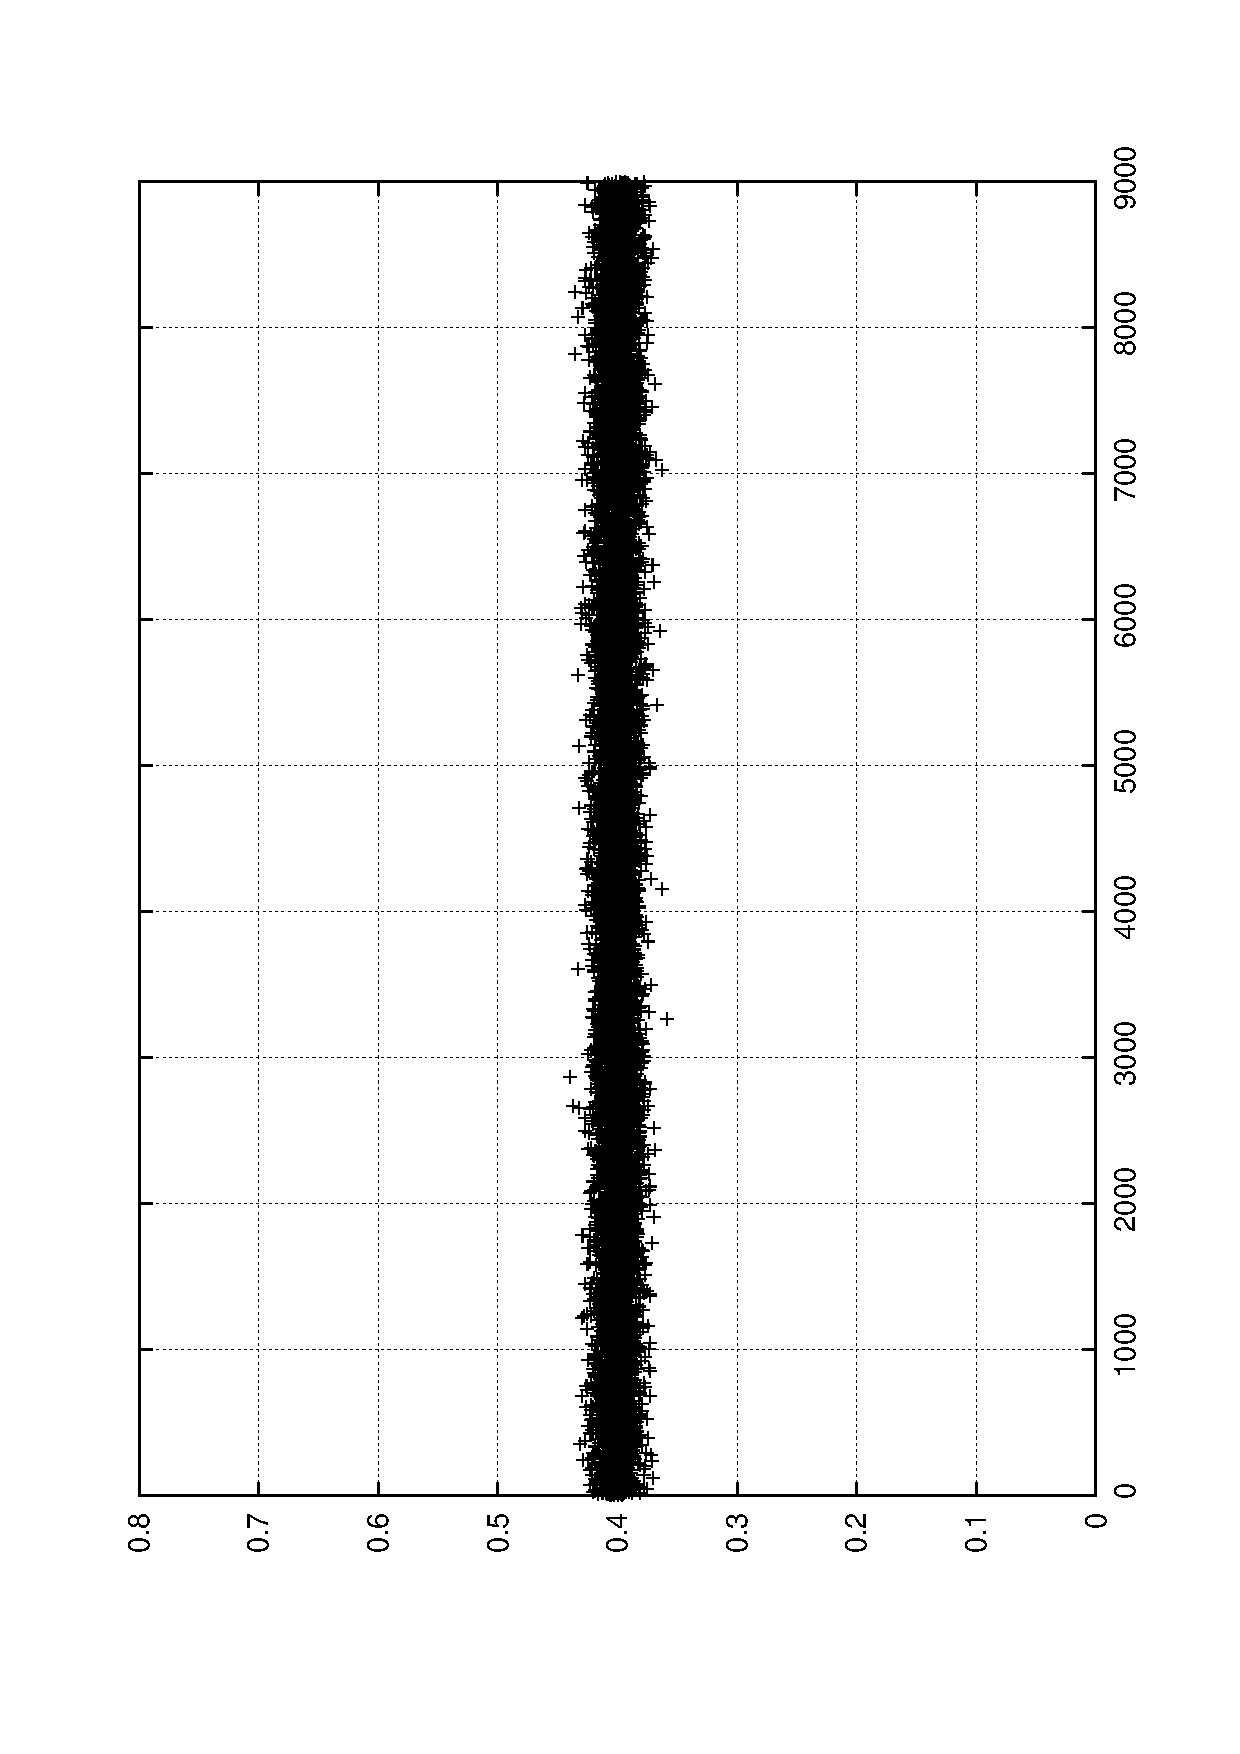
\includegraphics[scale=0.31]{trace-normal}
  \caption{Execution cost distribution for the scenario L1.}
  \label{fig:plotl1}
\end{figure}

\begin{figure}[h!t]
  \centering
  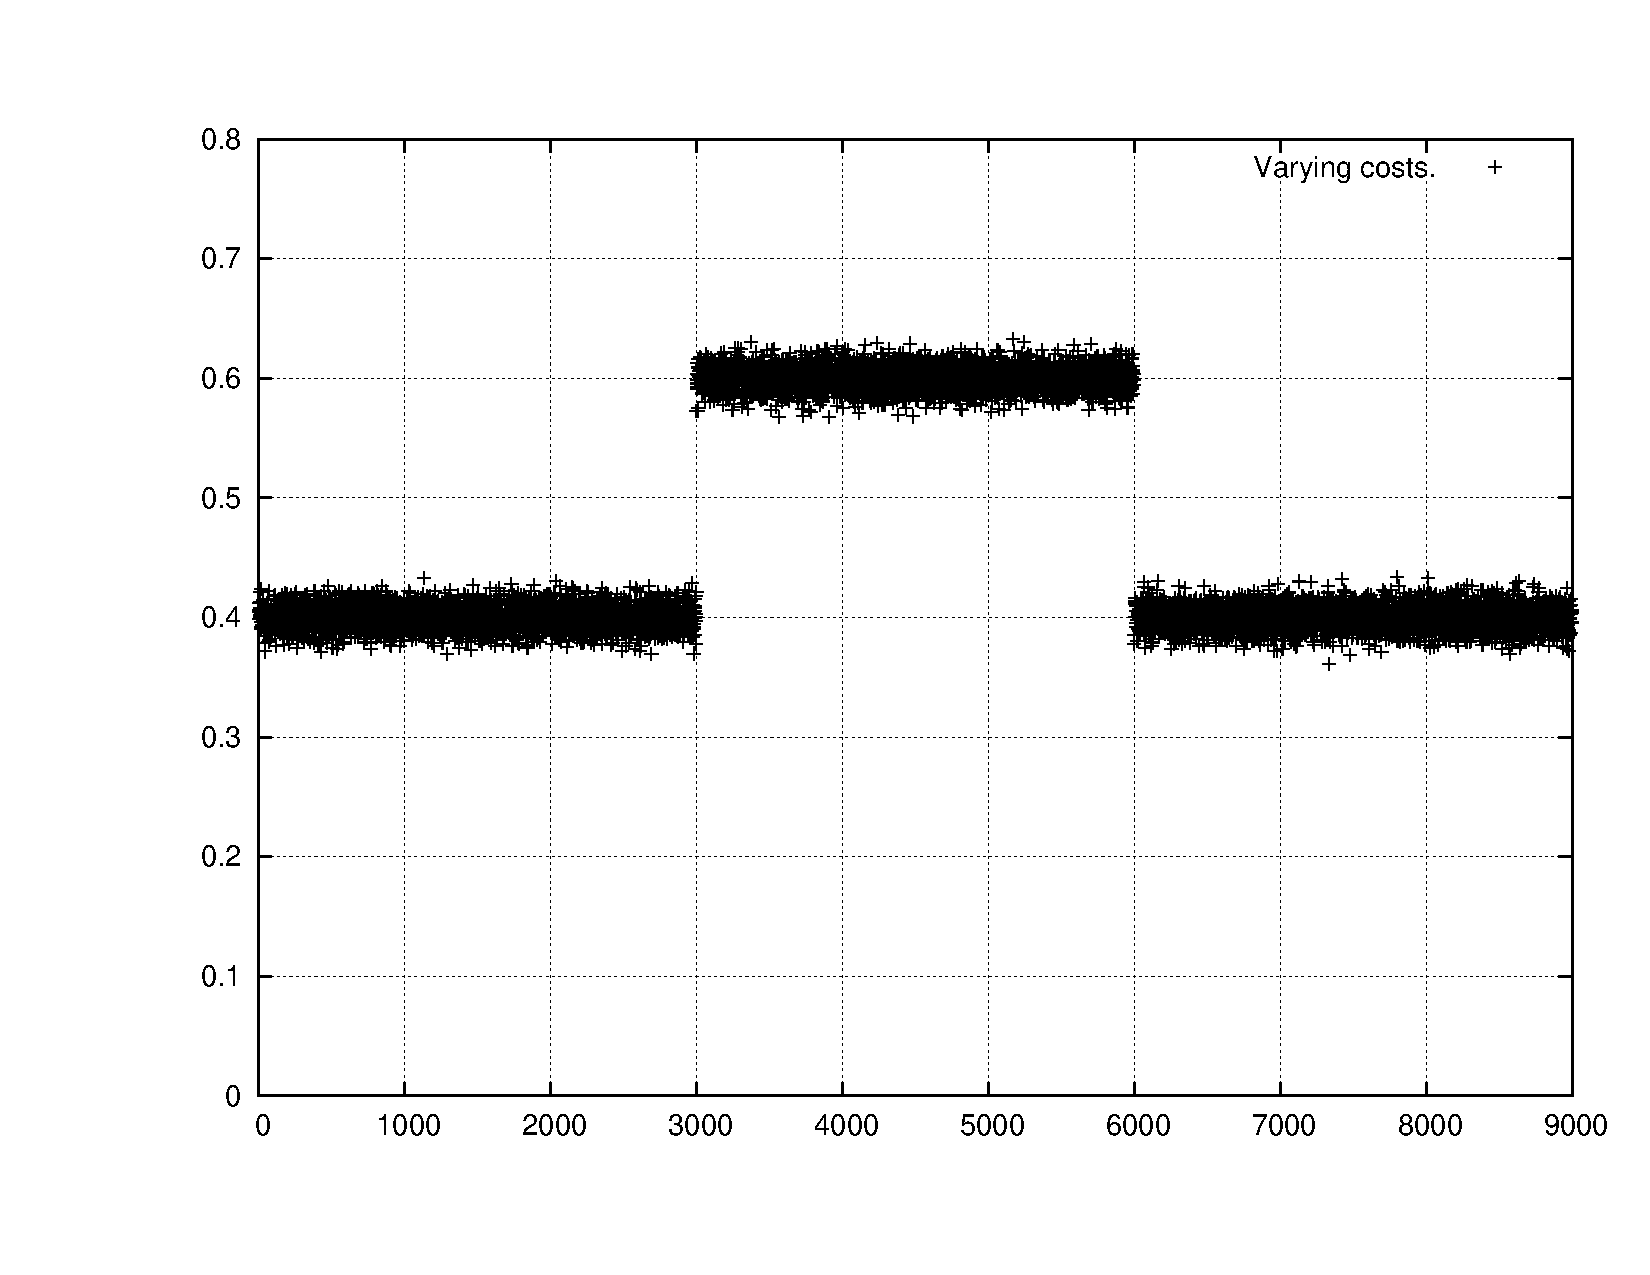
\includegraphics[scale=0.31]{trace-trifasico}
  \caption{Execution cost distribution for the scenario L2.}
  \label{fig:plotl2}
\end{figure}

\begin{figure}[h!t]
  \centering
  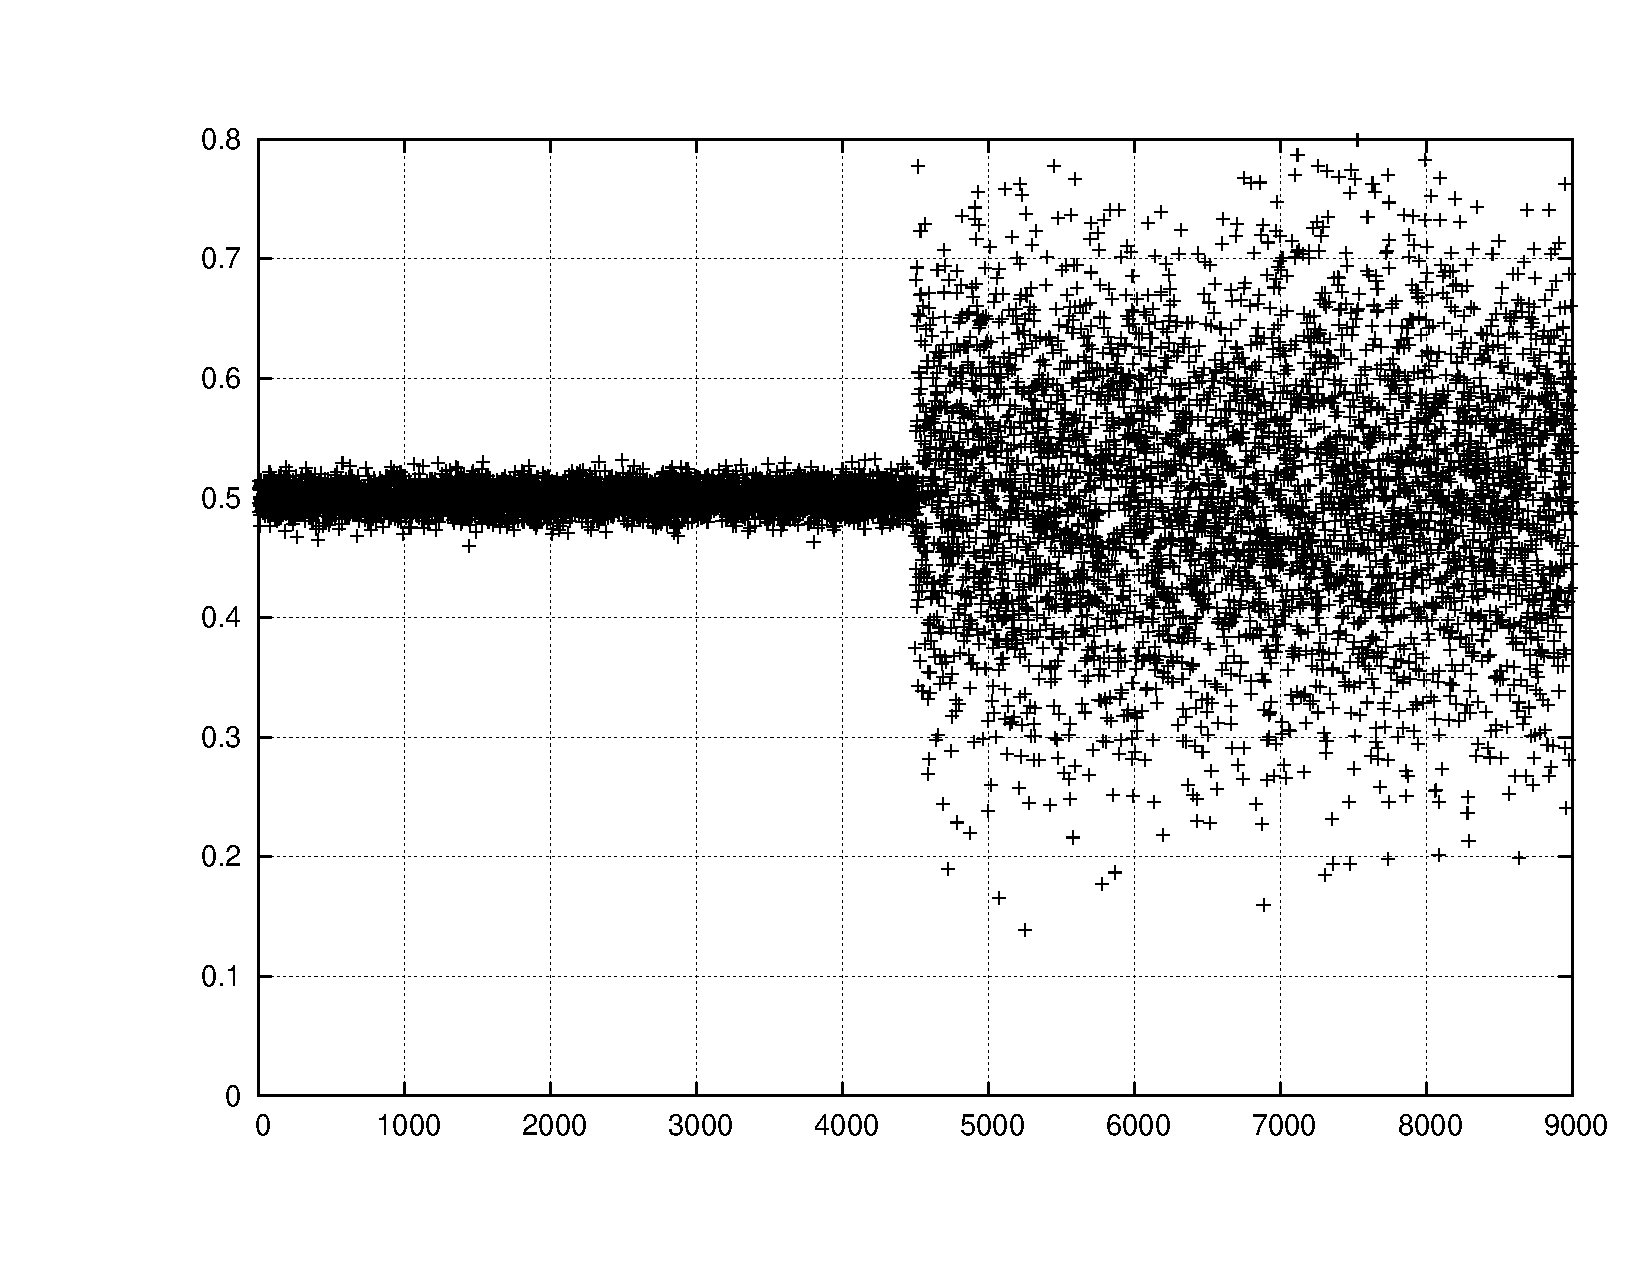
\includegraphics[scale=0.31]{trace-variance}
  \caption{Execution cost distribution for the scenario L3.}
  \label{fig:plotl3}
\end{figure}

\begin{figure}[h!t]
  \centering
  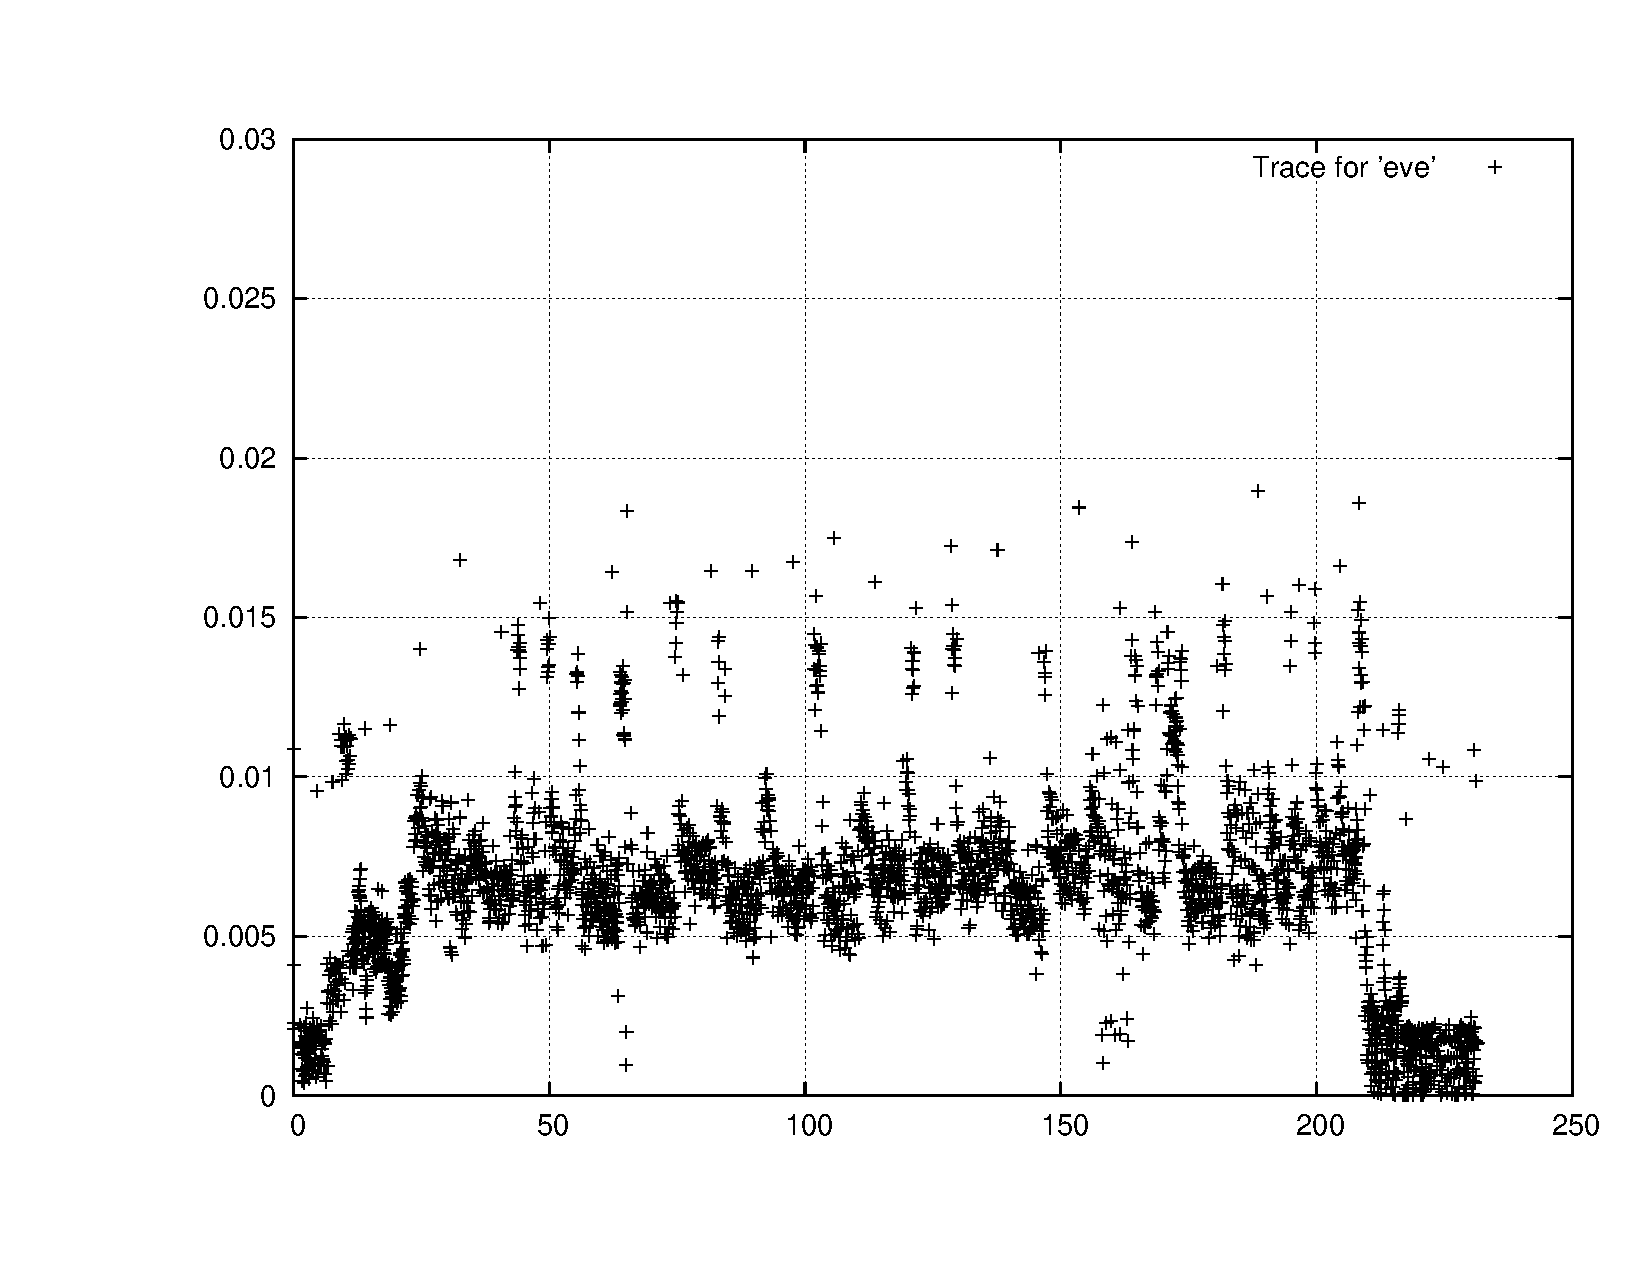
\includegraphics[scale=0.31]{trace-eve}
  \caption{Execution cost distribution for scenario L4.}
  \label{fig:plotl4}
\end{figure}

\Section{Simulation Results}
\label{sec:simulation-results}

As mentioned in section \ref{sec:configurations}, not all
configurations led to a performance difference. Section
\ref{sec:noDifference} first presents some comments on the reasons for
this behavior, and then, section \ref{sec:indiv-simul-results}
describes the results that highlight any differences in performance
between the hard and soft reservation schemes.

\SubSection{Equivalent Reservation Performance}
\label{sec:noDifference}

In configurations where expired tasks are not discarded, the system is
constantly overloaded or the server is underloaded both
reservation schemes performed equivalently. The explanation for this
behavior is given below.

\subsubsection{Discarding expired tasks}
\label{sec:disc-expir-tasks}

Consider a server $S = (Q,T)$ and that at time $t$ there is a
execution cost of $C$ to be served.  Since expired tasks are not
discarded, both hard and soft reservation servers will finish in at
least $\lfloor C/Q \rfloor T$ time units.  The only possible
difference is that a soft reservation server might spend this budget
before a hard reservation server can. In that case, the soft
reservation server may suffer some deadline postponements, but can
never finish executing a given job after an equivalent hard
reservation server. Hence, in general, not discarding expired tasks
makes soft and hard reservation completely equivalent.

\subsubsection{Overloaded system}
\label{sec:system-load}

When the system is always perfectly dimensioned or overloaded (there
is no system idle time) both reservation schemes are equivalent. This
is so because the soft server can only postpone its deadline to get
extra budget when there is free system time. Even if a soft
reservation server does exhaust its budget before its deadline, a
system under high load will usually have other higher-priority tasks
running and hence stopping the soft reservation server from using its
extra budget until the time gets closer to the server deadline (and by
then an equivalent hard reservation server would already be able to
use its budget).

\subsubsection{Underloaded server}
\label{sec:server-load}

Another scenario that does not highlight any significant differences
between hard and soft reservation is when the server load is low
enough that there is usually free budget upon completing a task. In
these situations both hard and soft reservation mechanisms are
equivalent, because, as less budget is needed per server period than
the server capacity, there will be very unfrequent budget
exhaustion.

\SubSection{Unequivalent Performance}
\label{sec:indiv-simul-results}

Reporting all possible situations that might highlight any differences
between soft and hard reservation is unpractical, so we chose a few
representative cases, already described in section
\ref{sec:configurations} as L1, L2, L3 and L4. Table \ref{tab:summary}
summarizes the simulation results.

\begin{table}[ht]
  \centering
  \begin{tabular}[t]{rrrrr} \hline
    \textsc{LS} & \textsc{RS} & \textsc{Mean RT} & \textsc{Mean WT} & \textsc{DMR (\%)} \\ \hline
    L1 & Soft & $5.1\times 10^{-1}$   & $2.5\times 10^{-1}$   & 5.4  \\
    L1 & Hard & $5.6\times 10^{-1}$   & $4.1\times 10^{-1}$   & 59.8 \\
    L2 & Soft & $4.8\times 10^{-1}$   & $1.7\times 10^{-1}$   & 14.4 \\
    L2 & Hard & $4.4\times 10^{-1}$   & $3.1\times 10^{-1}$   & 37.5 \\
    L3 & Soft & $5.7\times 10^{-1}$   & $2.4\times 10^{-1}$   & 5.1  \\
    L3 & Hard & $5.8\times 10^{-1}$   & $4.1\times 10^{-1}$   & 59.4 \\
    L4 & Soft & $6.5\times 10^{-3}$   & $2.2\times 10^{-3}$   & 0.1  \\
    L4 & Hard & $3.5\times 10^{-2}$   & $2.2\times 10^{-2}$   & 24.5 \\ \hline    
  \end{tabular}
  \caption{Result summary, with the mean response time (RT), wait time
  (WT) and deadline miss ratio (DMR) given for each load scenario (LS)
  and reservation scheme (RS).}
  \label{tab:summary}
\end{table}

\subsubsection{Scenario L1}
\label{sec:scenario-l1}

\begin{figure}[t]
  \centering
  \subfloat[Soft reservation.]{
    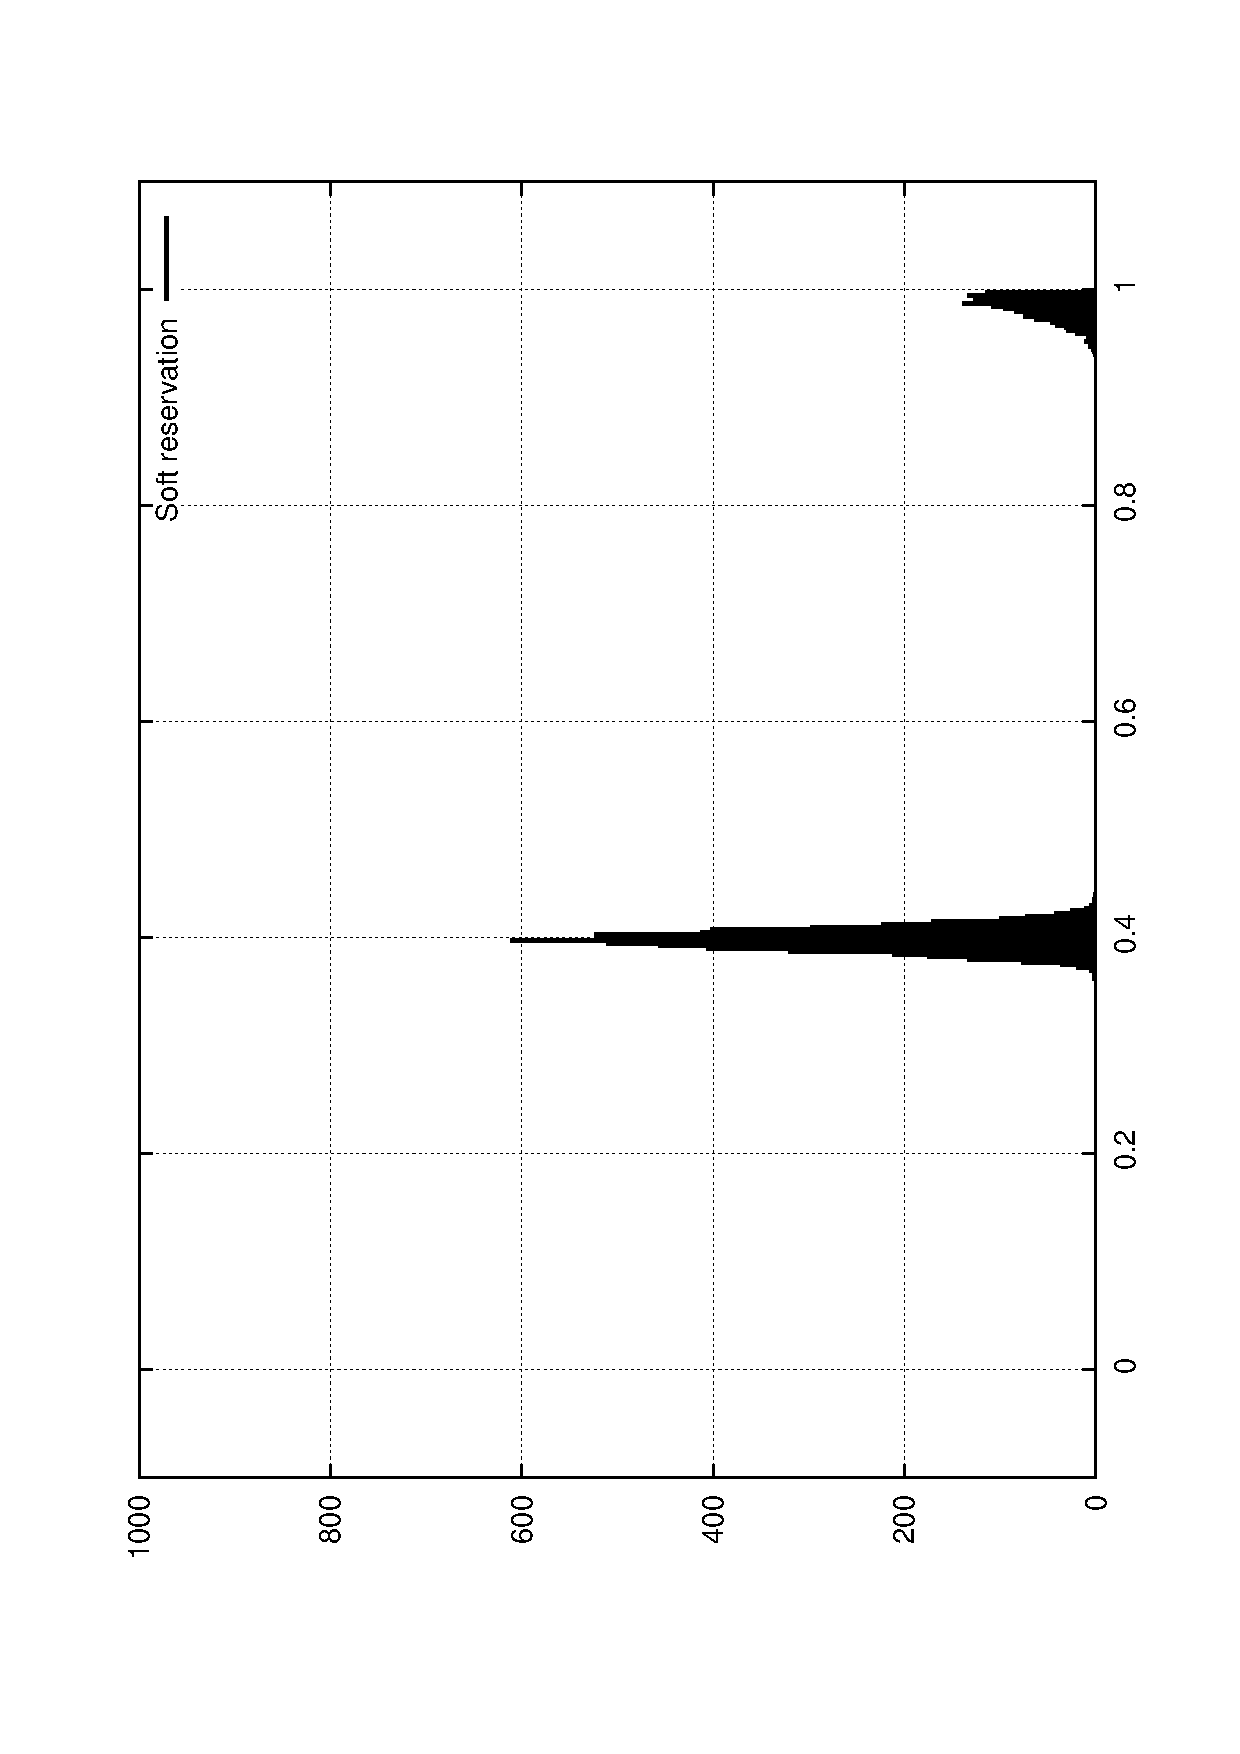
\includegraphics[scale=0.31]{rthisto1}
    \label{fig:soft-rth}
  }\\
  \subfloat[Hard reservation.]{
    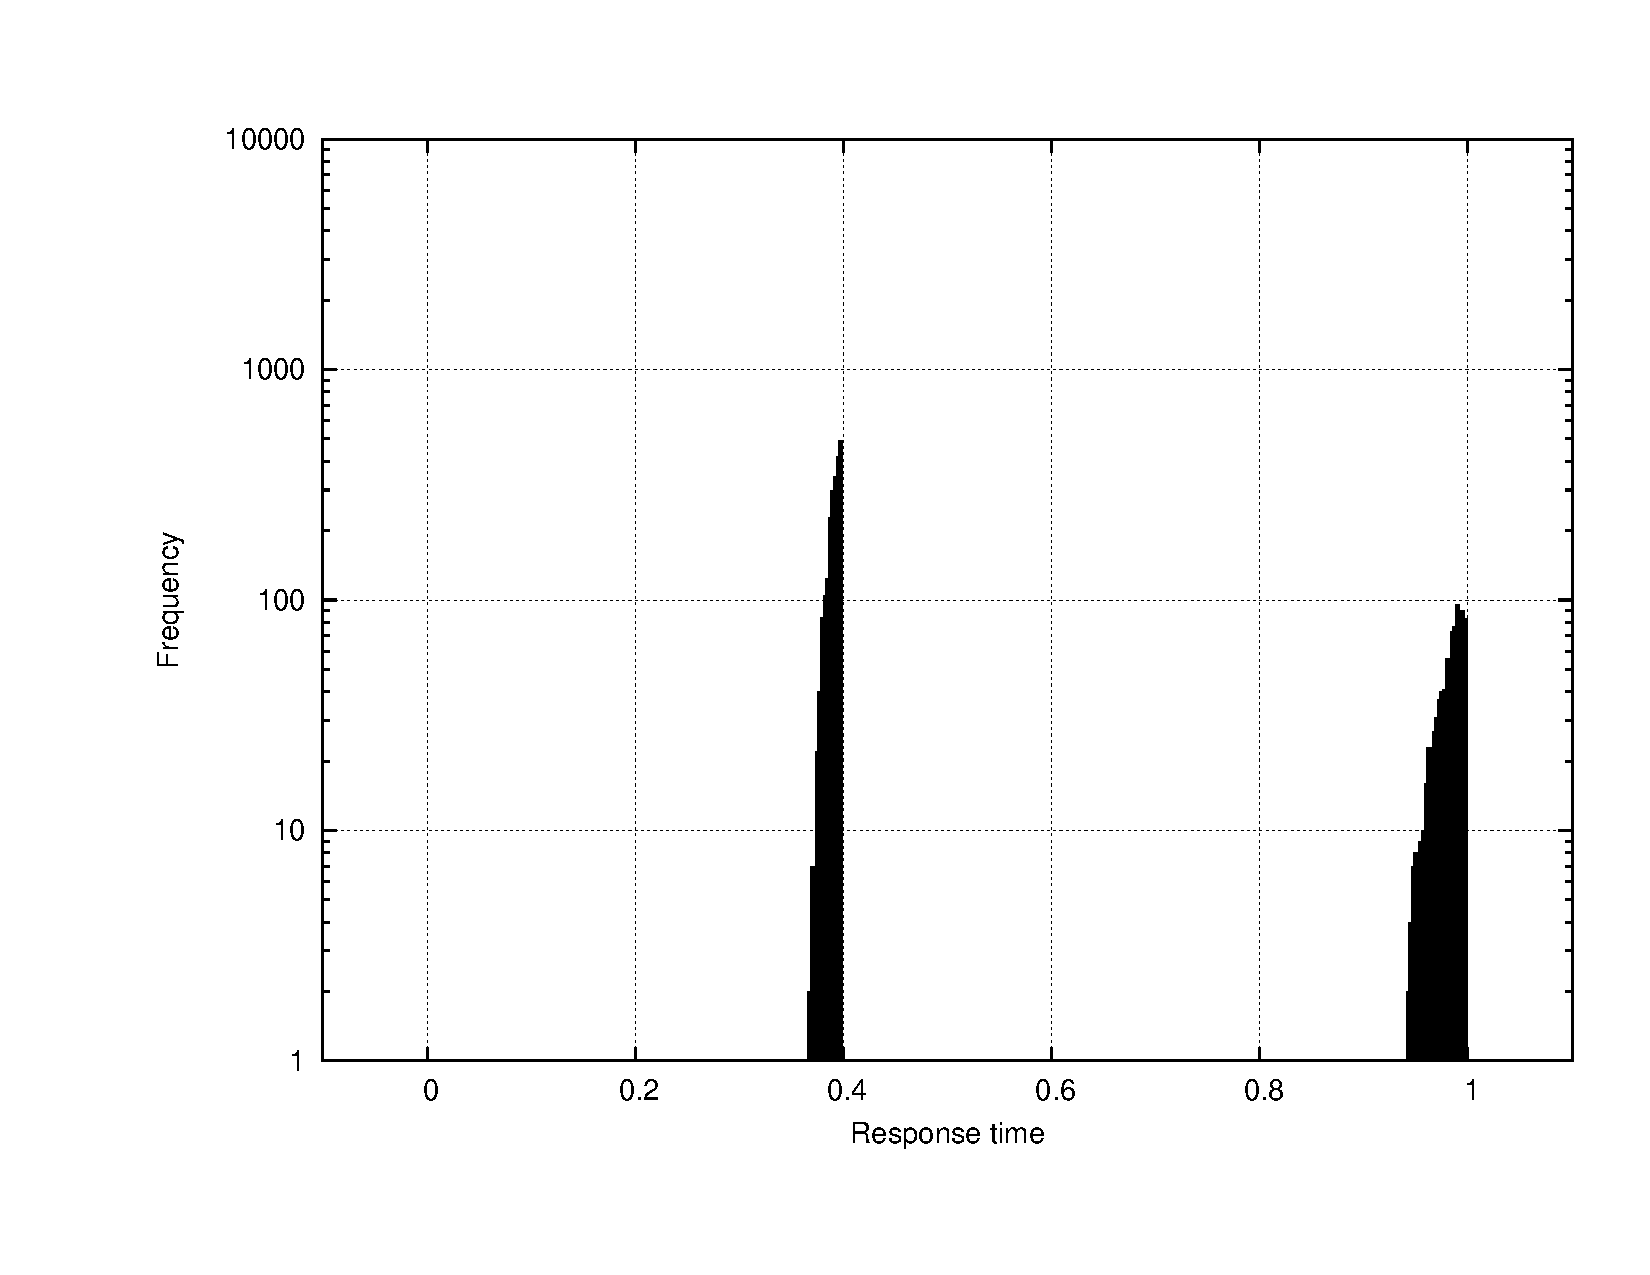
\includegraphics[scale=0.31]{rthisto2}
    \label{fig:hard-rth}
  }
  \caption{Response time histograms for scenario L1.}
  \label{fig:rth}
\end{figure}

\begin{figure}[t]
  \centering
  \subfloat[Soft reservation.]{
    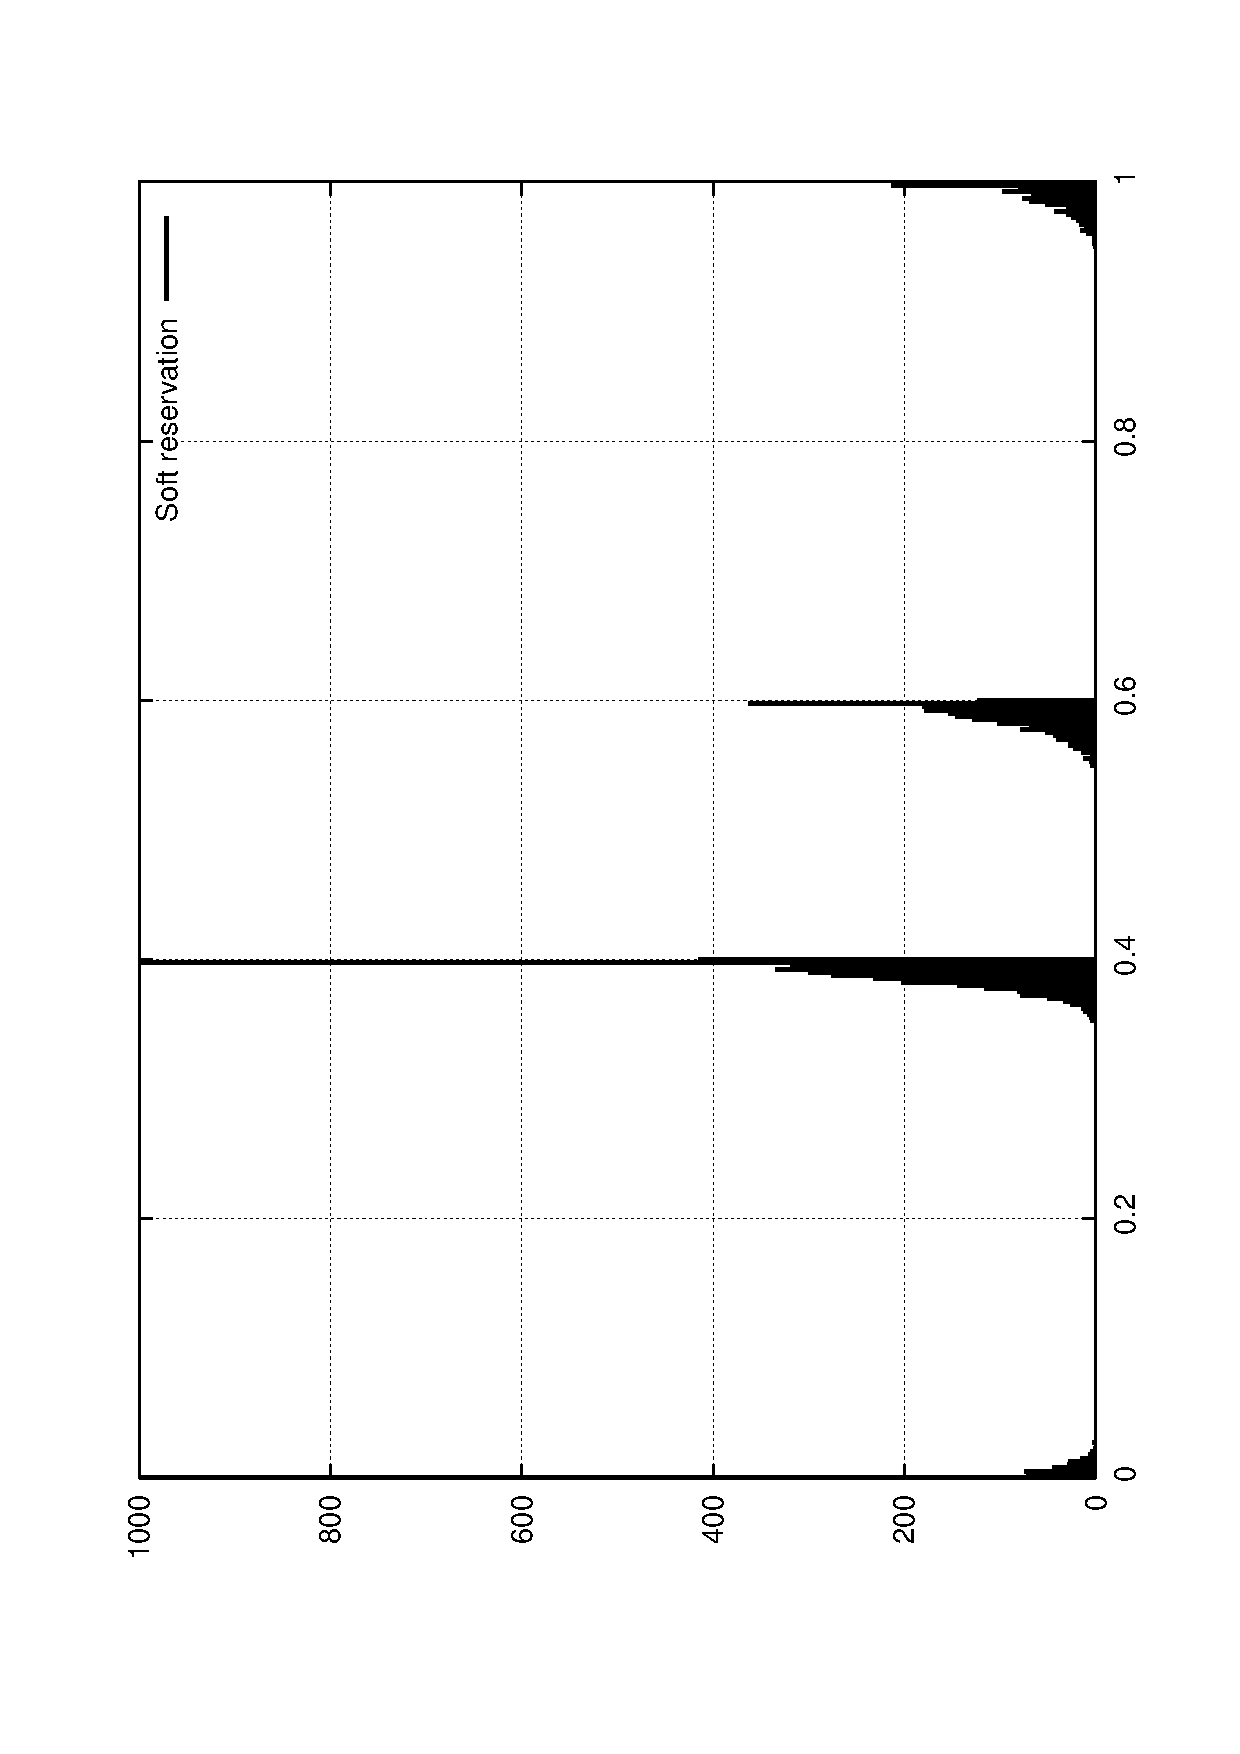
\includegraphics[scale=0.31]{dthisto1}
    \label{fig:soft-dth}
  }\\
  \subfloat[Hard reservation.]{
    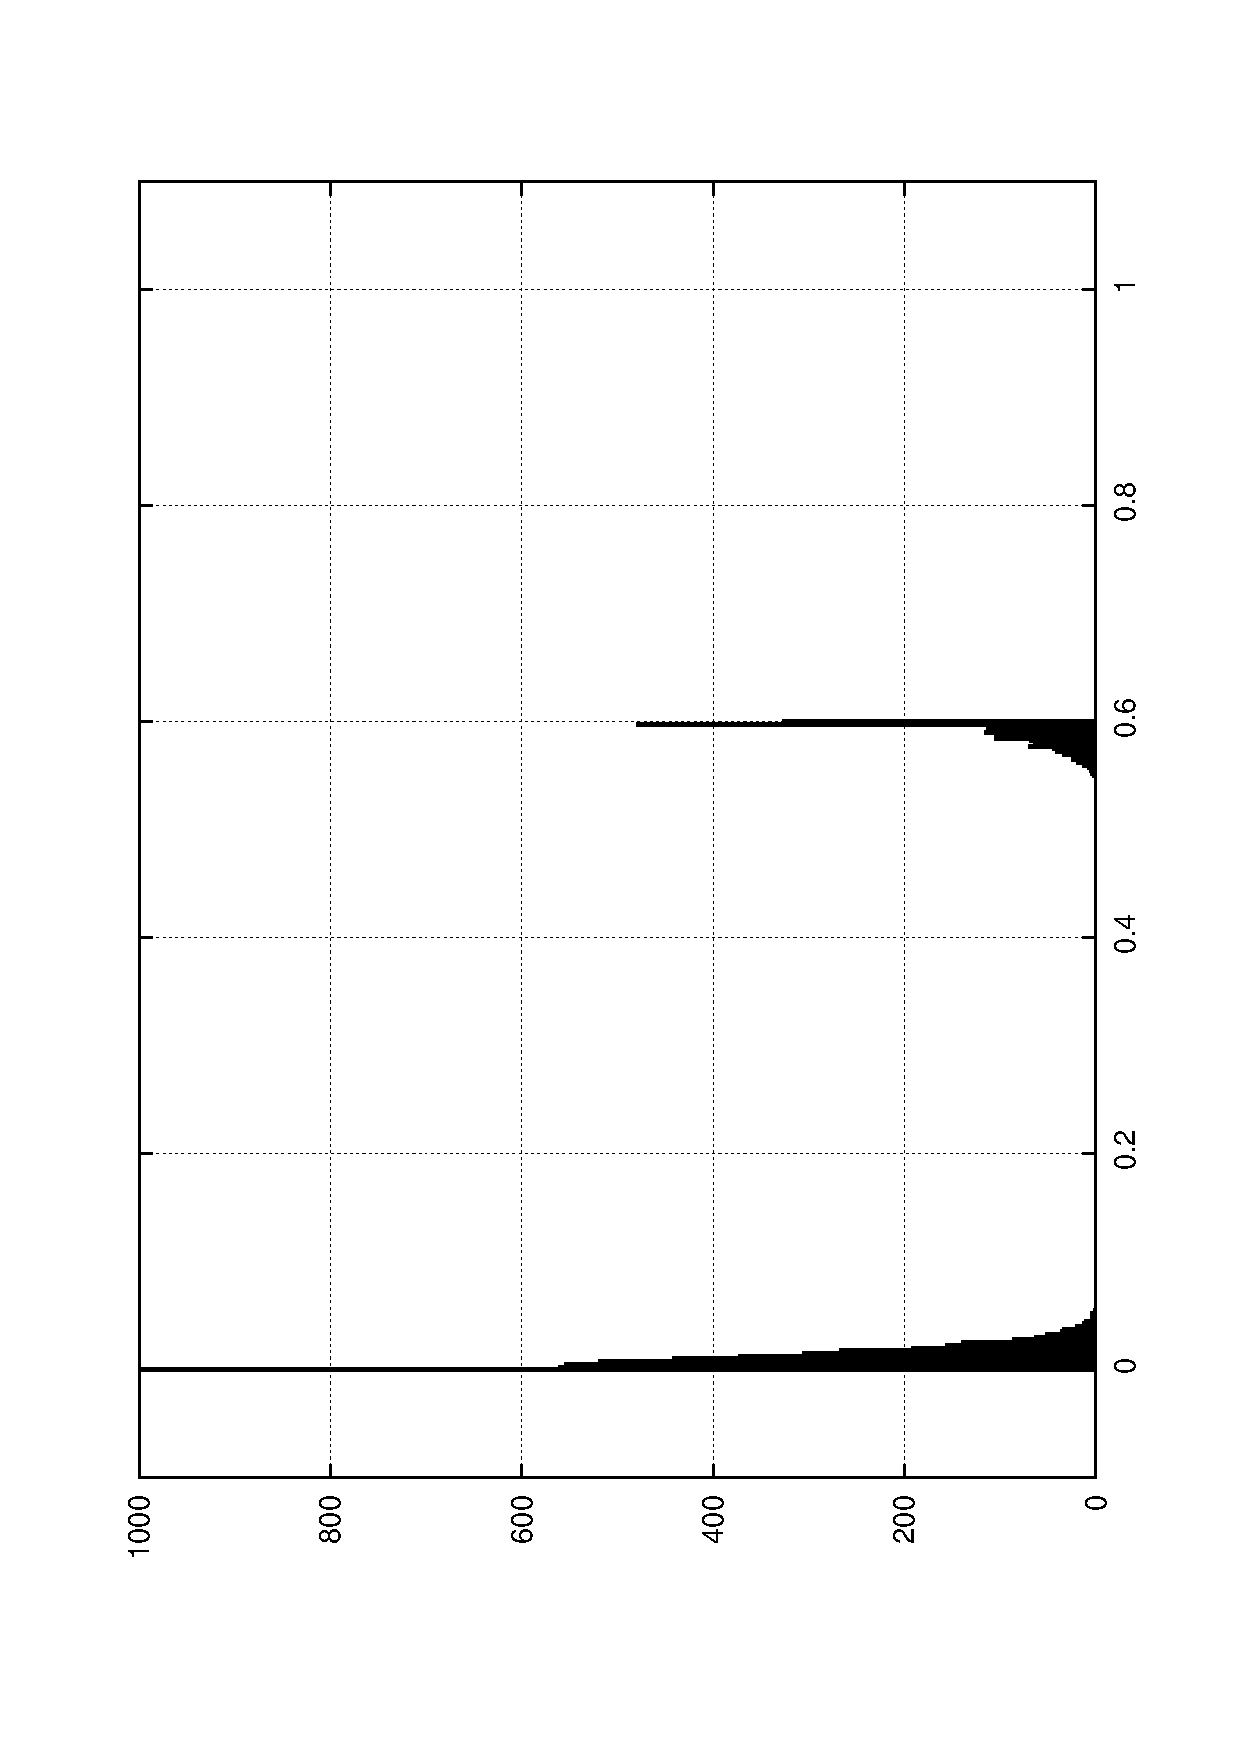
\includegraphics[scale=0.31]{dthisto2}
    \label{fig:hard-dth}
  }
  \caption{Wait time histograms for scenario L1.}
  \label{fig:dth}
\end{figure}

A general idea of how soft and hard reservation can behave might be
given by a simulation with the costs in scenario L1. Since the
distribution of the execution costs is normal and constant throughout
the simulation, the distribution of response and wait times is better
characterized by a histogram. Figures \ref{fig:rth} and \ref{fig:dth}
show histograms of response time and waiting time for soft and hard
reservation on a system running tasks from scenario L1. The horizontal
axis represents each possible value, in time units, for the response
or waiting times, while the vertical axis counts how many times each
such value has actually occurred. In this scenario, the soft
reservation server missed 5.4\% of the deadlines and the hard
reservation server missed 59.8\%, as seen in Table
\ref{tab:summary}. As can be seen, both the histograms for the soft
reservation server have higher peaks on smaller response and wait
times than their hard reservation equivalents. This behavior indicates
that the soft reservation server is likely a better way of employing
system resources.

\begin{figure}[t]
  \centering
  \subfloat[Soft reservation.]{
    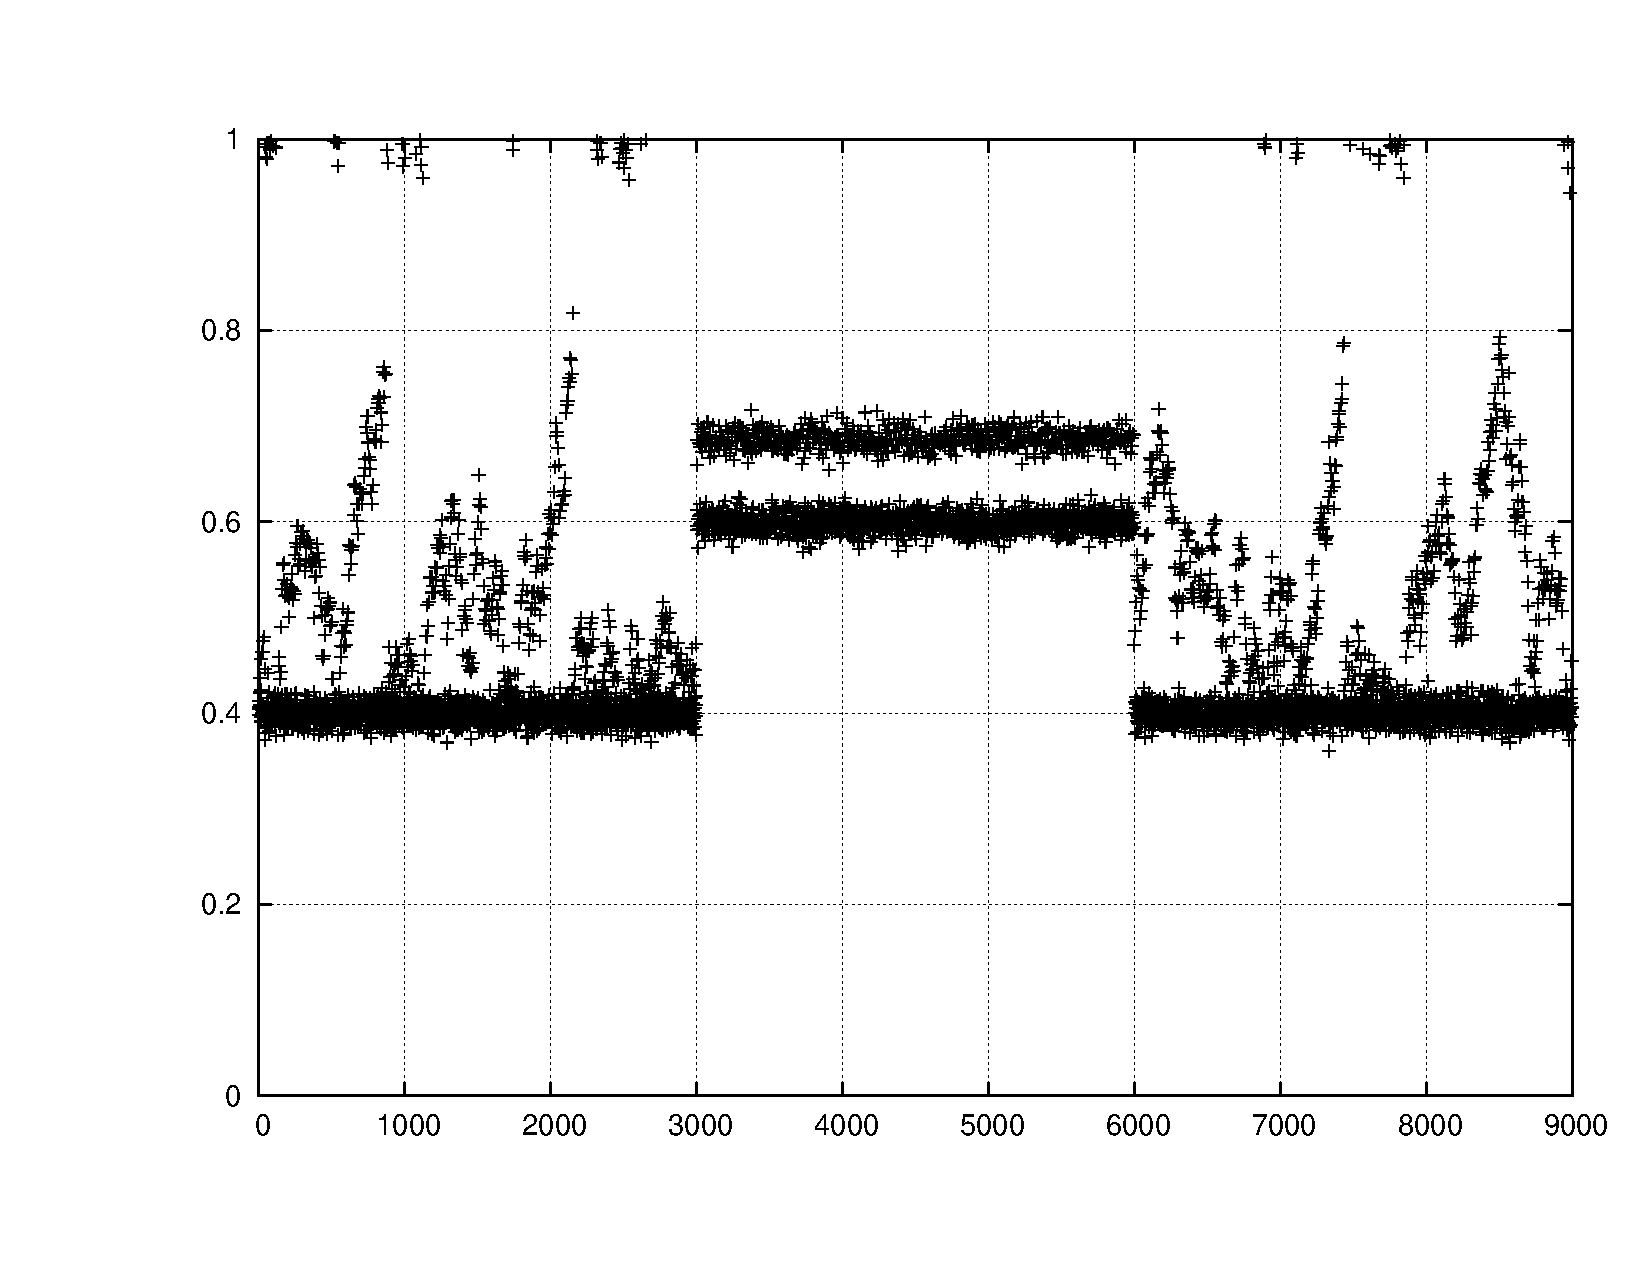
\includegraphics[scale=0.31]{trifasico-1}
    \label{fig:soft-trifasico}
  }\\
  \subfloat[Hard reservation.]{
    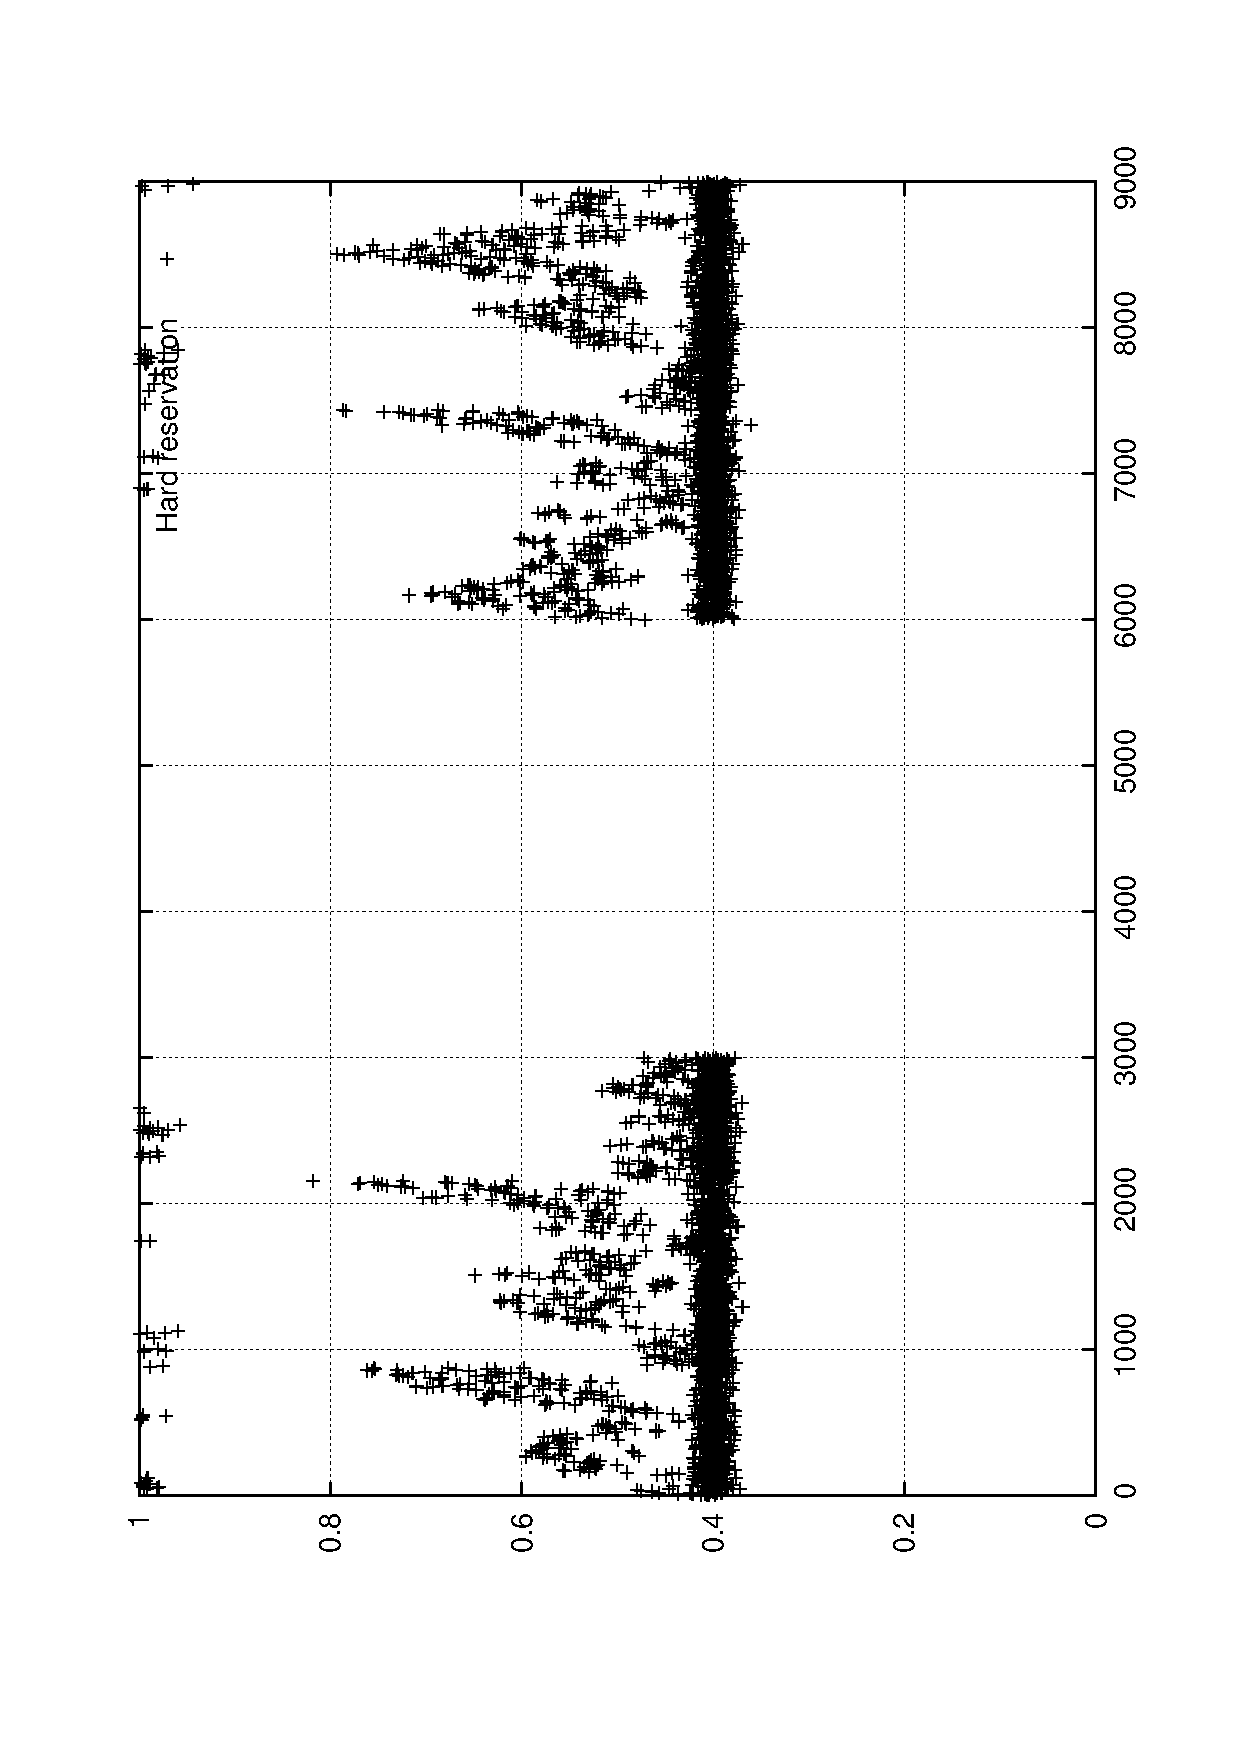
\includegraphics[scale=0.31]{trifasico-2}
    \label{fig:hard-trifasico}
  }
  \caption{Response times for scenario L2.}
  \label{fig:trifasico}
\end{figure}

\subsubsection{Scenario L2}
\label{sec:scenario-l2}

The effect of markedly different execution costs over time is also
interesting. In this experiment, the task set first starts with a
correctly dimensioned server, until time $t=3000$, when the mean costs
for the tasks rise suddenly. After a while, the costs return to
normal. Figure \ref{fig:trifasico} shows the response times for this
scenario. The wait times, not shown specifically, follow a similar
pattern. Each point $(x,y)$ in the graph represents a task that,
finishing at time $x$, had a response time of $y$. Therefore, when the
same area is denser in one graph (as happens in the middle section of
this scenario), it means that the server with a higher density
completed more tasks. This kind of graph, while not precisely
describing the distribution of the response times, shows a clear
picture of hoe they change over time. As this figure shows, in the
heavily loaded part only the soft reservation server can finish tasks
that need more than the server budget. This suggests that the soft
reservation server is better able to cope with run-time varying
requirements. Also, when the load comes back down there is no extra
cost for the soft reservation server, and its response times are
equivalent to the response times for the hard reservation
server. Thus, in variable environments a soft reservation scheme seems
more suitable for situations where the application load changes over
time. This information might be relevant for soft real-time systems
running some adaptation mechanism, such as the one described in
\cite{abeni.ea05:qos}.

\begin{figure}[t]
  \centering
  \subfloat[Soft reservation.]{
    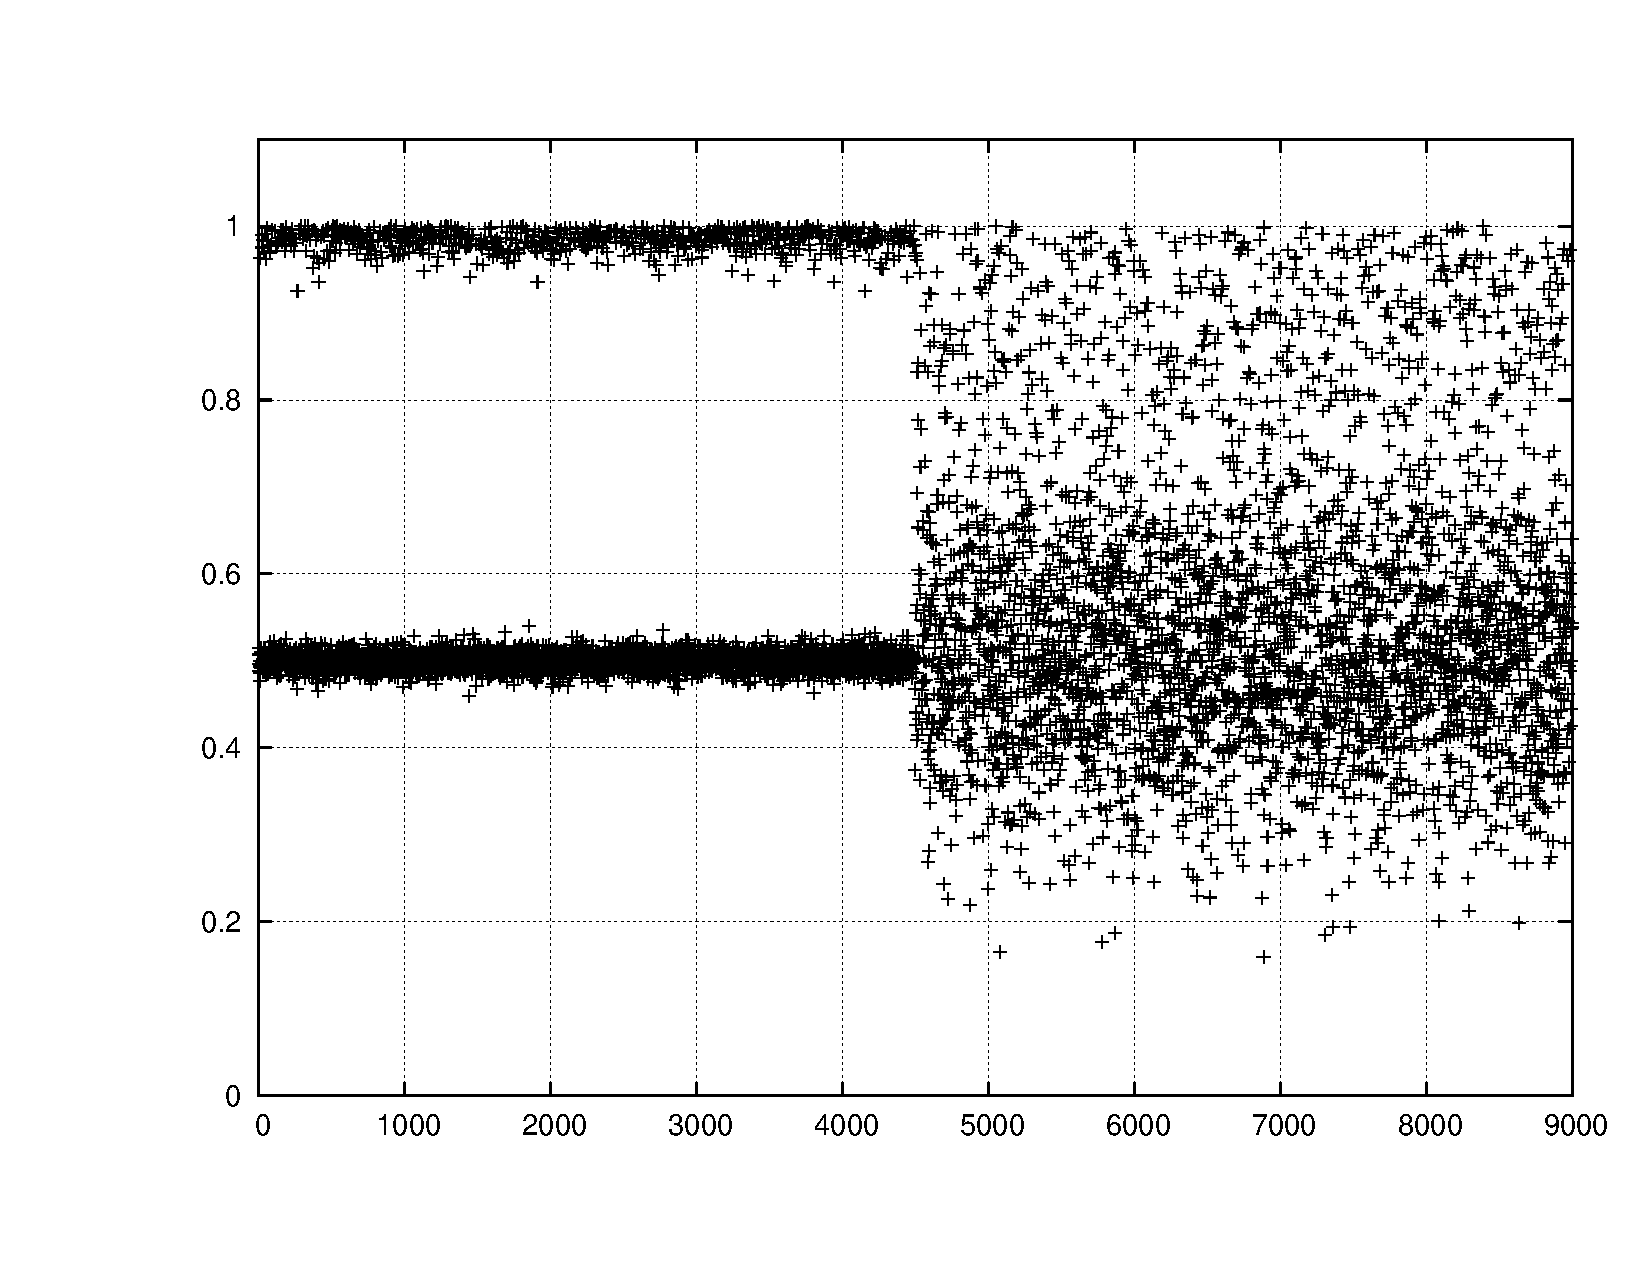
\includegraphics[scale=0.31]{variance-1}
    \label{fig:soft-variance}
  }\\
  \subfloat[Hard reservation.]{
    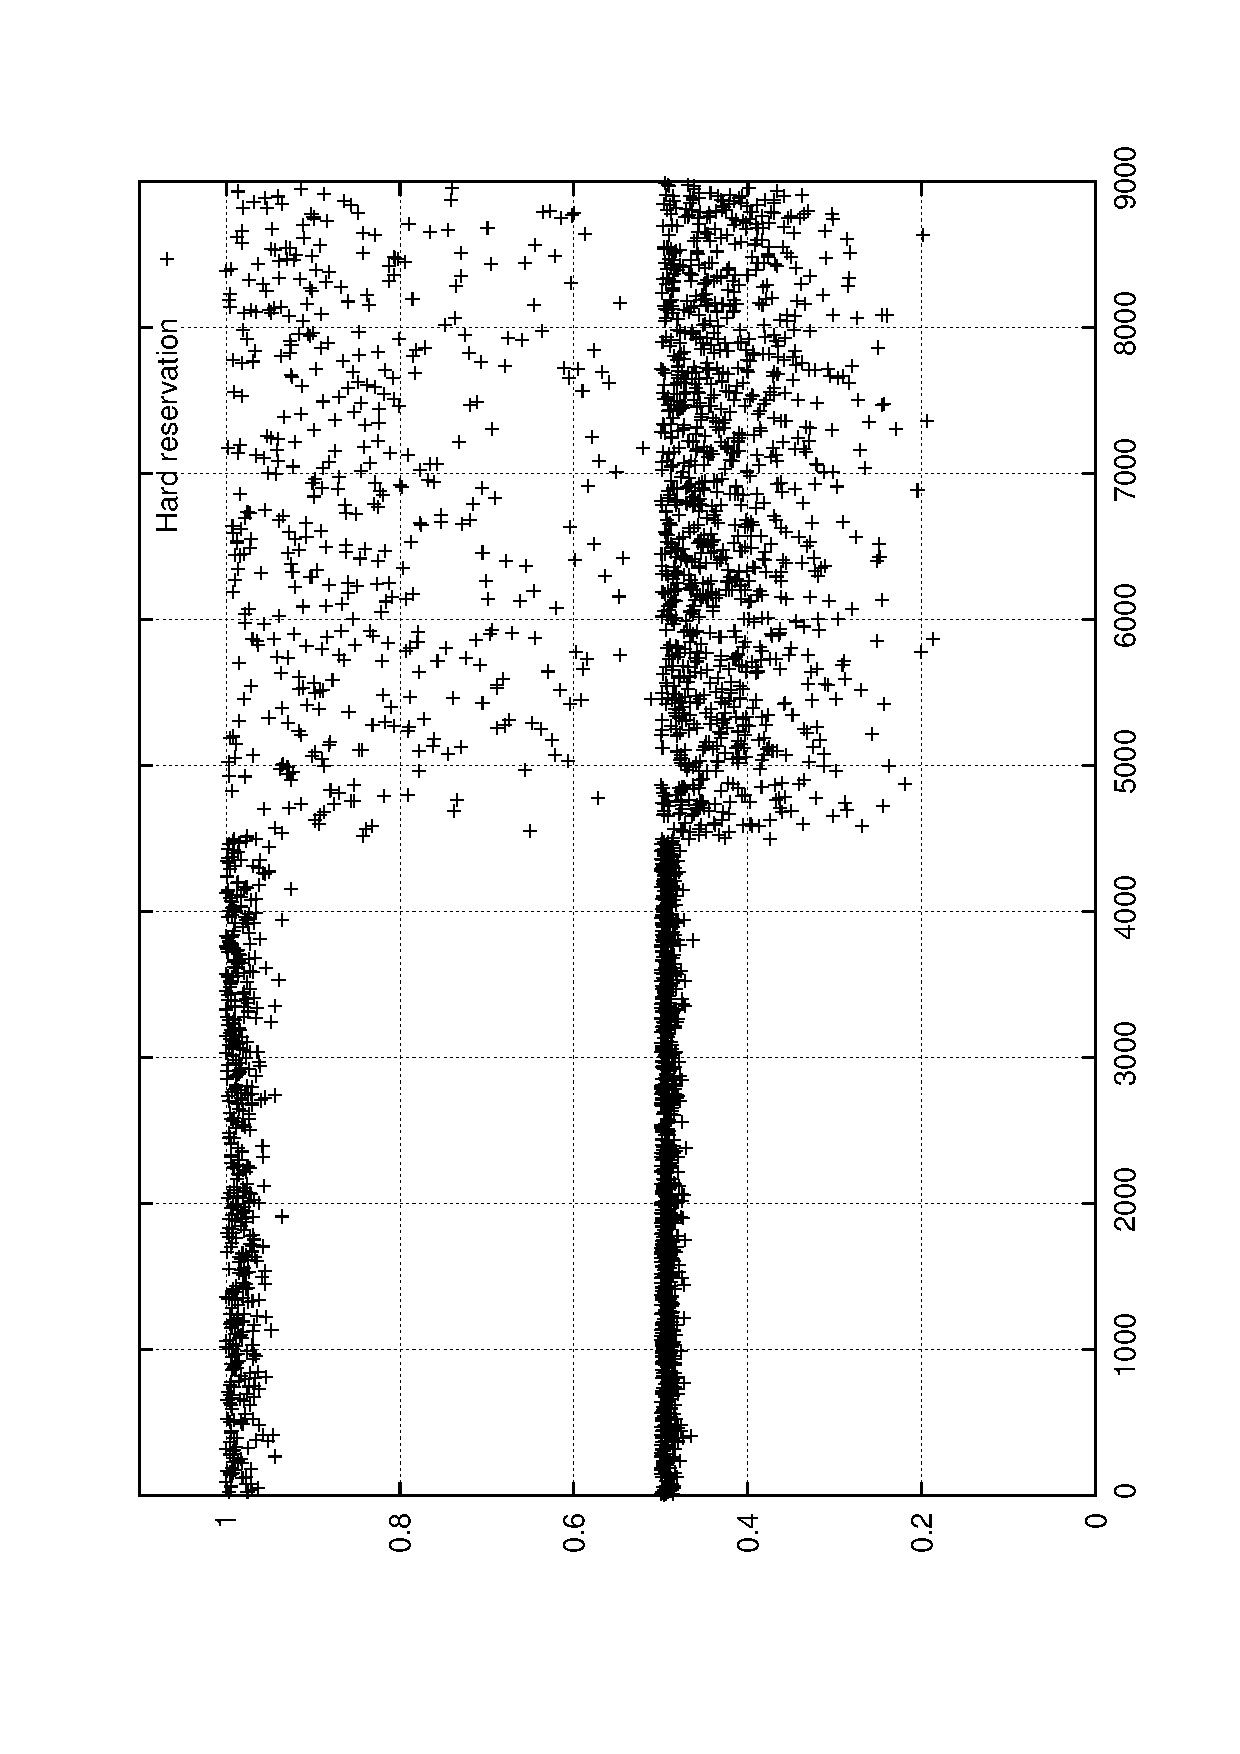
\includegraphics[scale=0.31]{variance-2}
    \label{fig:hard-variance}
  }
  \caption{Response times for scenario L3.}
  \label{fig:variance}
\end{figure}

\subsubsection{Scenario L3}
\label{sec:scenario-l3}

Another possible situation in which a RBS server might have its
responsivity compromised is when dealing with tasks having a high
variance in its execution costs. Scenario L3 was designed to test this
possibility. This might happen because to serve tasks with
unexpectedly high costs, a soft reservation server might need to
postpone its deadline too much, while a hard reservation server would
be more prudent and instead discard these costly outliers, being more
performant in the remaining time. In this experiment the hard
reservation server missed 59.39\% of the deadlines, while the soft
reservation only missed 5.19\%. Figure \ref{fig:variance} shows the
response times for this experiment. The wait times behaved similarly
and were omitted from this paper. As can be easily seen, in the
higher variance part the soft reservation server manages to finish
many more tasks in a short amount of time than the hard reservation
server, thus behaving better on task sets with a high variance.

\begin{figure}[t]
  \centering
  \subfloat[Soft reservation.]{
    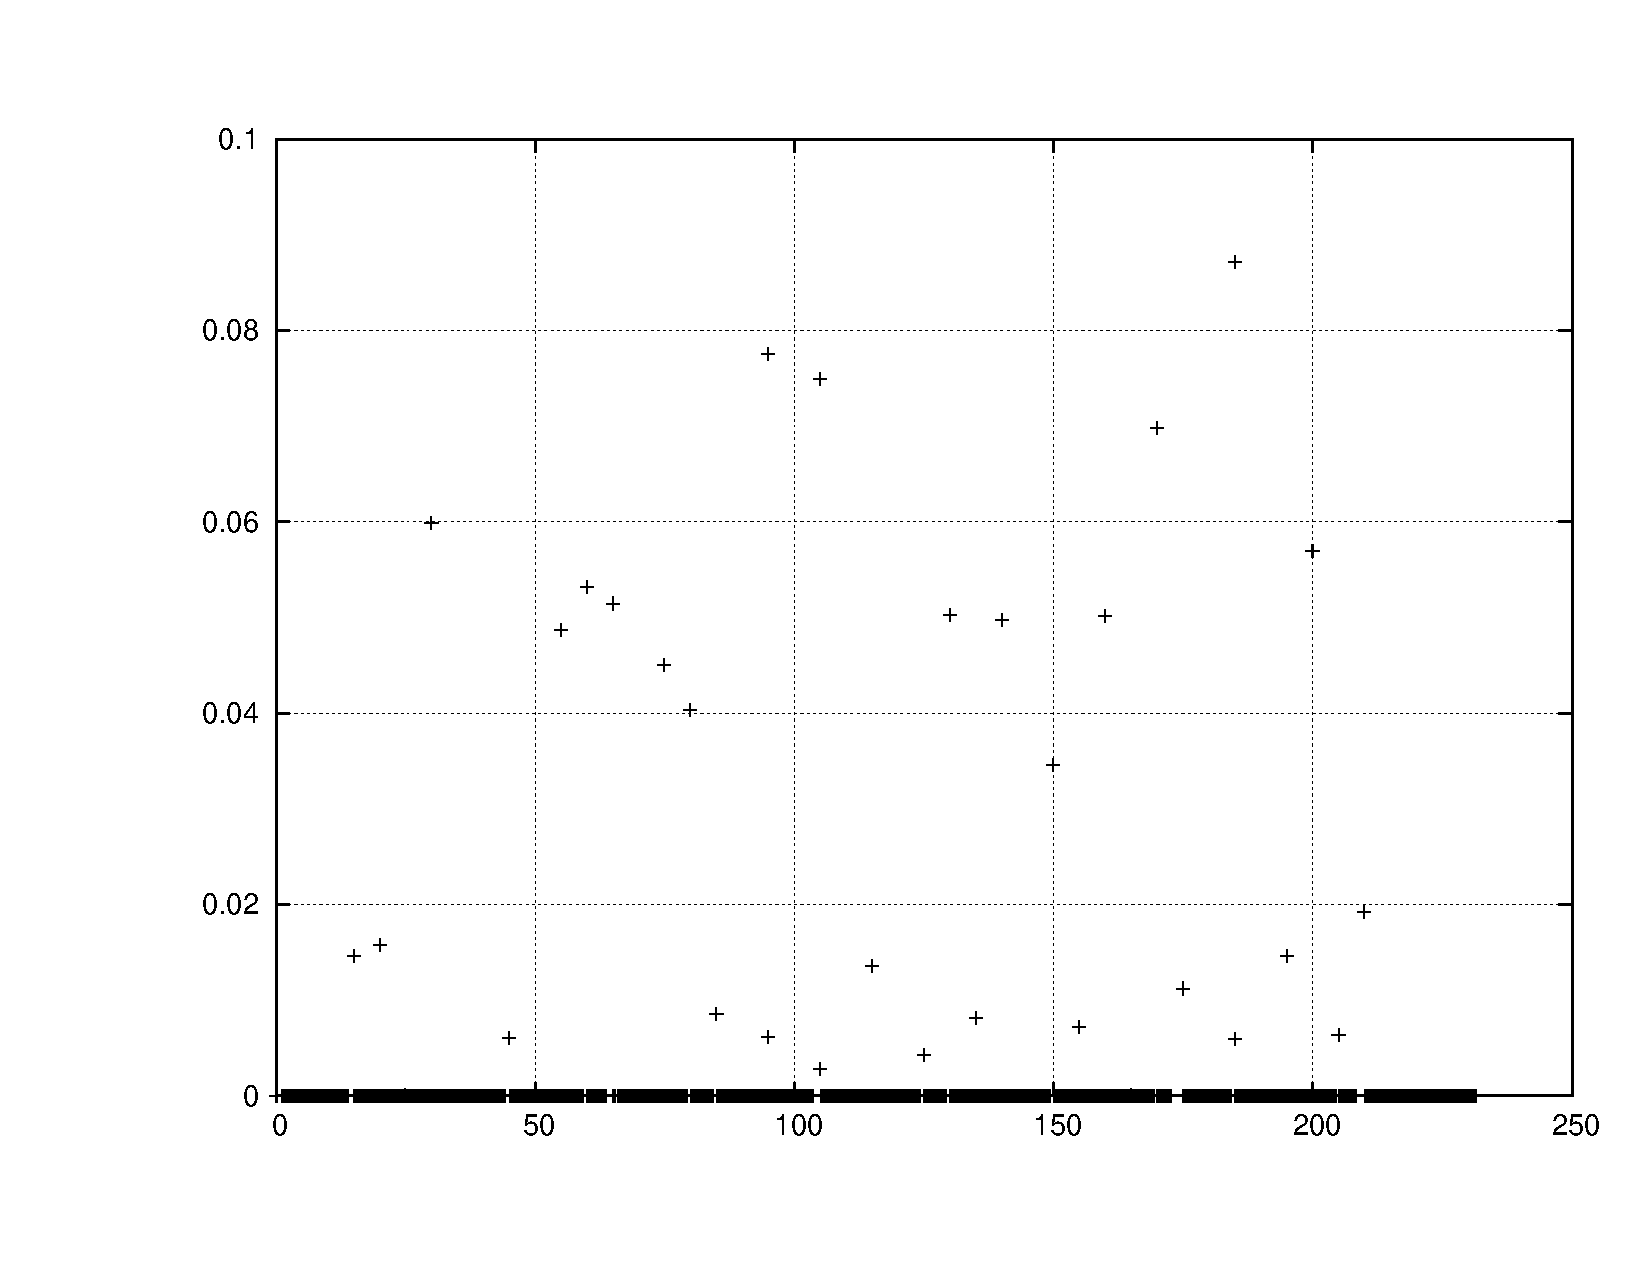
\includegraphics[scale=0.31]{eve-1}
    \label{fig:soft-eve}
  } \\
  \subfloat[Hard reservation.]{
    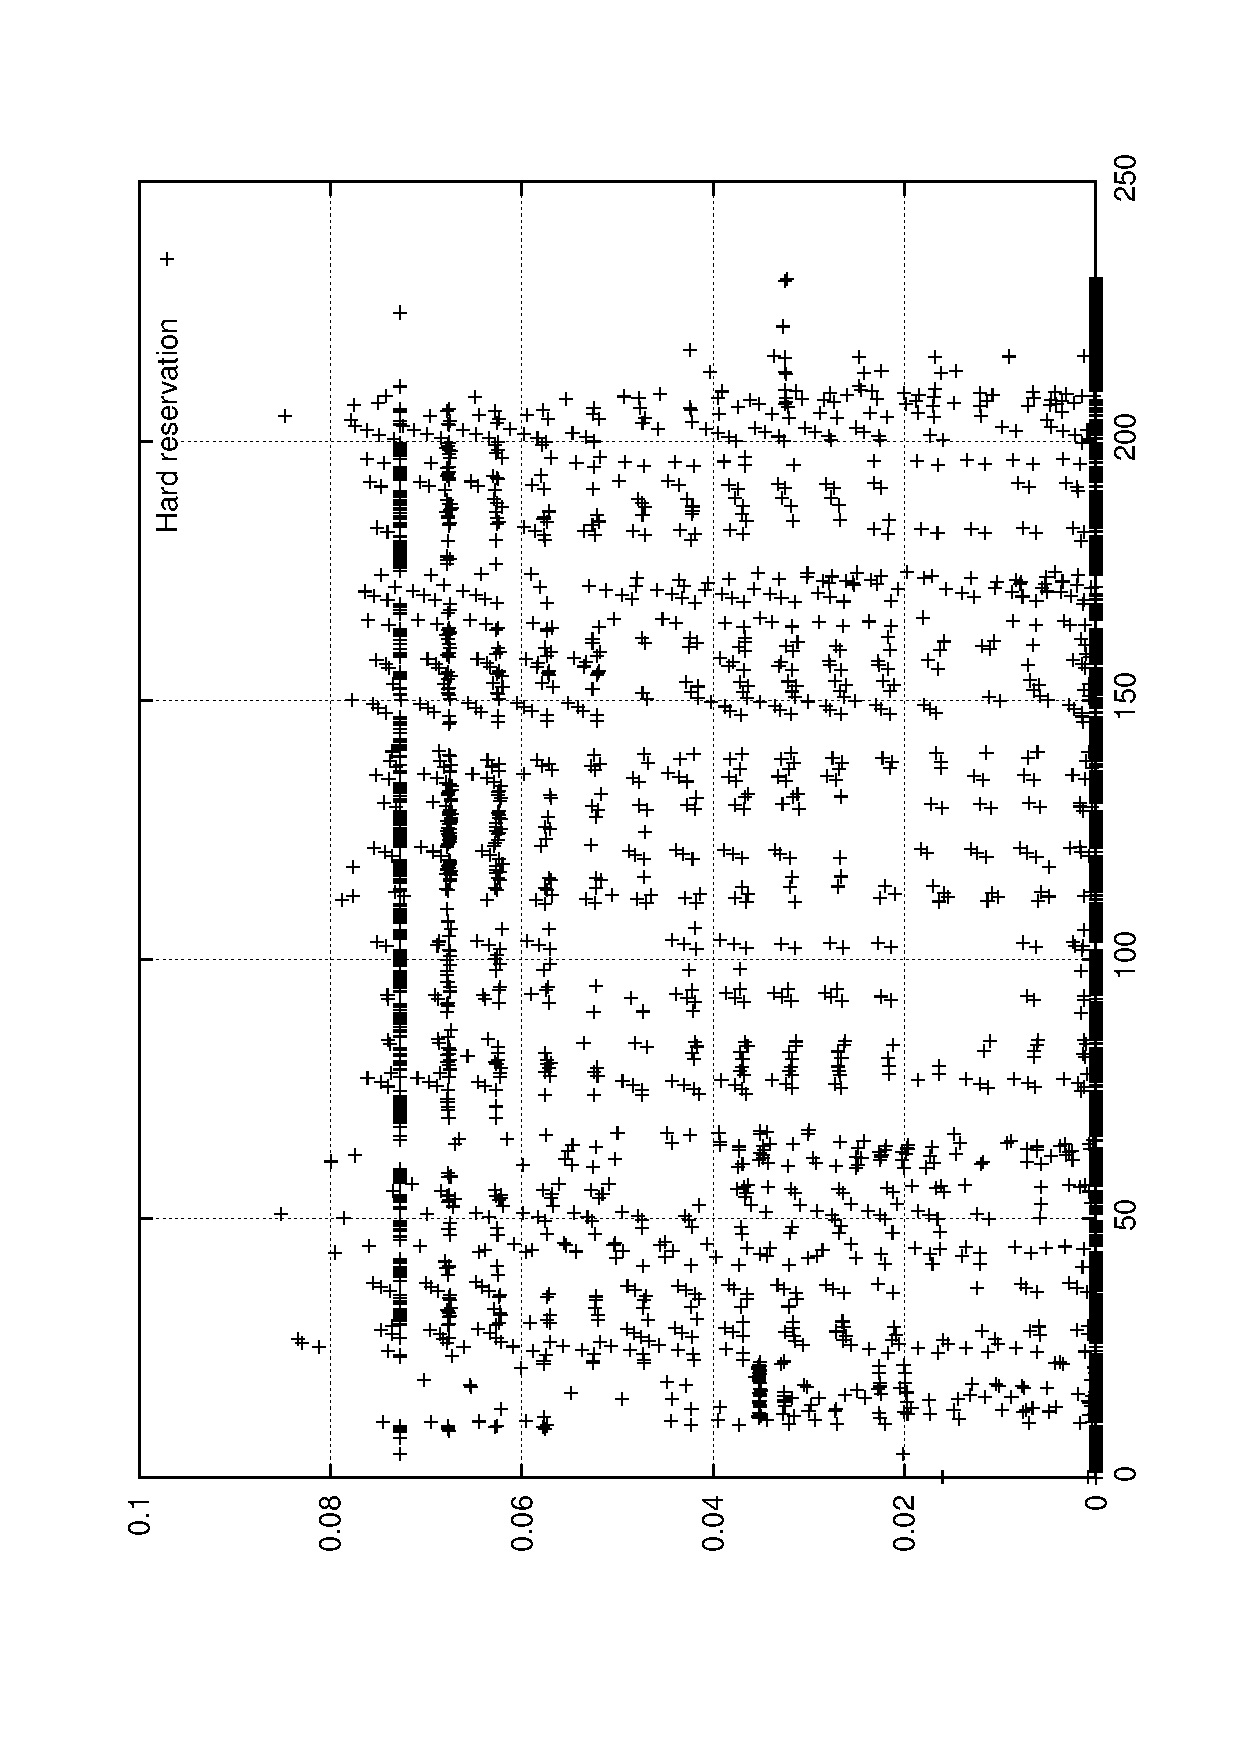
\includegraphics[scale=0.31]{eve-2}
    \label{fig:hard-eve}
  }
  \caption{Wait times for scenario L4, the movie trace.}
  \label{fig:eve}
\end{figure}

\subsubsection{Scenario L4}
\label{sec:scenario-l4}

Another very important test case is whether, in non-synthetic tasks,
the performance characteristics we observed are reproduced. In this
experiment, we ran both a soft reservation server and a hard
reservation server on scenario L4. Figure \ref{fig:eve} shows the wait
time for both a hard and a soft reservation servers running this task
set. As can be easily seen, the wait time for the hard reservation
server is always higher than for the soft reservation server,
sometimes high enough that the task has already missed its deadline by
the time it starts executing. This might account for the fact that, as
can be seen in Table \ref{tab:summary}, the soft reservation server
only missed 0.1\% of the deadlines, while the hard reservation server
missed 24.54\%. This result seems, at first, counter-intuitive, since
the soft reservation server, by delaying its deadline whenever the
execution costs are too high, can have an arbitrarily low priority. On
the other hand, the same task will take more overall time to be served
with a hard reservation server, since it will have to wait for
capacity replenishment before continuing execution. Therefore, on
average, the soft reservation scheme seems more responsive.

\Section{Conclusion}
\label{sec:conclusion}

Reservation-based scheduling has been increasingly used to support
modern soft and hard real-time systems. Some implementations of both
hard and soft reservation schemes have been proposed in real-time
operating systems.

In this paper we have conducted a systematic study on the performance
of soft and hard reservation schemes. As we have seen, both
reservation schemes present equivalent performance for several
configurations, but, using simple but illustrative load scenarios, we
have shown that soft reservation schemes outperforms the hard one by
having shorter response times, substantially shorter wait times and
significantly smaller deadline miss ratios. This results suggests that
soft reservation servers are better able to use system resources
without either compromising overall system schedulability or task
quality of service. We believe that the results and scenarios
presented here can be used by people designing reservation-based
algorithms or real-time operating systems to support some important
implementation decisions.

\bibliographystyle{latex8}
\bibliography{bib}
\end{document}
